\documentclass[a4paper]{article}
\usepackage{bchow}
\usepackage{hhline}

%font
\setmainfont{KpLight}
\setsansfont{CMU Bright}[Scale=MatchLowercase]
\setmonofont{KpMono}
\setmathfont{KpMath-Light.otf}[math-style=ISO,bold-style=TeX,StylisticSet={1,3,4},CharacterVariant={2,3,6}]

\renewcommand{\familydefault}{\rmdefault}

%image path
\graphicspath{{./images/}}

\begin{document}
\title{{ECOS3010}\\{\normalsize{Monetary Economics -- Notes}}}
	\author{Brendan Chow}
	\abstract{Based on the lecture notes by A/Prof Stella Huangfu}
	\affiliation{
	Student at the University of Sydney\\
	\href{https://xagill.com/}{Website}\\
	\href{https://www.linkedin.com/in/brendanchow/}{LinkedIn}\\
	\href{https://github.com/ARocketdog}{GitHub}\\
	}
	\emailAdd{brendanchow@xagill.com}
	\maketitle
	\newpage
	\pagestyle{fancynotes}
%start document
\section{A Simple Model of Money}
\subsection{Introduction}
	\begin{itemize}
		\item Money has always been important to people and to the economy.
		\item Money has a long history.
		\begin{itemize}
			\item Commodity money: shells, beads, cigarettes, silver, gold,\ldots
		\item Fiat money: paper currency \( \rightarrow \) intrinsically useless
		\item Emoney: debit card, smart card, ecash,\ldots
		\end{itemize}
		\item  Are we headed for a cashless society?
		\item Why do we need money?
		\begin{itemize}
			\item Lack of double coincidence of wants.
			\item Lack of record-keeping or credit:\@ money is MEMORY!
		\end{itemize}
		\item Functions of money:
		\begin{itemize}
			\item a medium of exchange: primary function;
			\item a unit of account;
			\item a store of value.
		\end{itemize}
		\item A suitable framework to study issues related to money: the overlapping generations (OLG) model.
		\begin{itemize}
			\item highly tractable;
			\item an elegant way to introduce money;
			\item dynamic.
		\end{itemize}
	\end{itemize}
\subsection{Enviroment of the Model}
	\begin{itemize}
		\item The economy begins in period 1 and runs forever: \( t = 1, 2, \dots , \infty \).
		\item Individuals live for two periods: \textit{young} and \textit{old}.
		\item In period \( t \), \( N_t \) individuals are born. In the first period, \( N_0 \) initial old.
		\item In each period \( t \), \( N_t \) young individuals and \( N_{t-1} \) old individuals.
		\item Each individual receives \( y \) units of goods when young and nothing when old.
		\item Here is a summary of the model so far:
	\end{itemize}
	\begin{table}[h]\centering
		\begin{tabular}{|c|c|c|c|c|c|}
			\hline
			Generation & t=1 & t=2 & t=3 & t=4 & \( \rightarrow \) \\ \hline
			0 & 0 &  &  &  &  \\ \hline
			1 & \( y \) & 0 &  &  &  \\ \hline
			2 &  & \( y \) & 0 &  &  \\ \hline
			3 &  &  & \( y \) & 0 &  \\ \hline
			\( \downarrow \) &  &  &  &  \( \cdots \) & \( \cdots \) \\ \hline
		\end{tabular}
	\end{table}
	\begin{itemize}
		\item Preferences:
		\begin{itemize}
			\item Individuals of all future generations value consumption both when young and when old.
			\item Initial old value consumption only when old.
		\end{itemize}
	\end{itemize}
	\begin{itemize}
		\item Three assumptions about an individual's utility
		\begin{enumerate}[label=\textbf{\arabic*.}]
			\item Utility is increasing with the consumption.
		\begin{marginfigure}
			\centering
			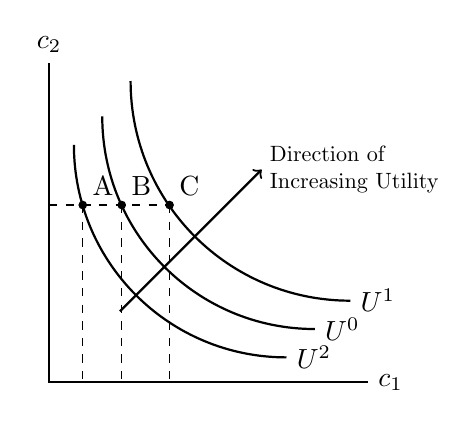
\begin{tikzpicture}[scale=0.45]
				\draw [thick] (0,9) node[above]{\(c_2\)}--(0,0)--(9,0) node[right]{\(c_1\)};
				\draw [thick] (1.5,7.5) to [out=-90,in=180] (7.5,1.5) node[right]{\( U^0 \)};
				\draw [thick] (2.3,8.5) to [out=-90,in=180] (8.5,2.3) node[right]{\( U^1 \)};
				\draw [thick] (0.7,6.7) to [out=-90,in=180] (6.7,0.7) node[right]{\( U^2 \)};
				\draw [thick, ->] (2,2)--(6,6) node[right, align=left,scale=0.8]{Direction of\\Increasing Utility};
				\draw [dashed] (0,5)--(3.4,5);
				\draw [dashed] (3.4,5)--(3.4,0);
				\draw [dashed] (2.05,5)--(2.05,0);
				\draw [dashed] (0.95,5)--(0.95,0);
				\filldraw [black] (0.95,5) circle (3pt) node[above right]{A};
				\filldraw [black] (2.05,5) circle (3pt) node[above right]{B};
				\filldraw [black] (3.4,5) circle (3pt) node[above right]{C};
 			\end{tikzpicture}
			\caption{Increasing utility}
		\end{marginfigure}
		\item Individuals value some consumption in both periods of life: the indifference curves never cross either axis.
		\item Diminished marginal rate of substitution
		\end{enumerate}
	\end{itemize}
\subsection{Centralised Solution: the Golden Rule Allocation}
	\begin{itemize}
		\item Suppose there is a central planner who can allocate the available goods among the young and the old in each period.
		\item Let \( (c_{1,t}, c_{2,t+1}) \) note the consumption bundle by individuals born in period \( t \).
		\item Resource constraint in period \( t \) is
		\[
			N_t c_{1,t} + N_{t-1} c_{2,t} \leq N_t y.
		\]
		\item Suppose for now that for all \( t \),
		\begin{itemize}
			\item the population is constant: \( N_t = N \)
			\item we foucs on stationary allocations where \( c_{1,t} = c_1 \) and \( c_{2,t} = c_2 \).
		\end{itemize}
		\item Resource constraint simplifies to
		\[
			c_1 + c_2 \leq y.
		\]
		\item Graphically the feasible set is
		\begin{marginfigure}
			\centering
			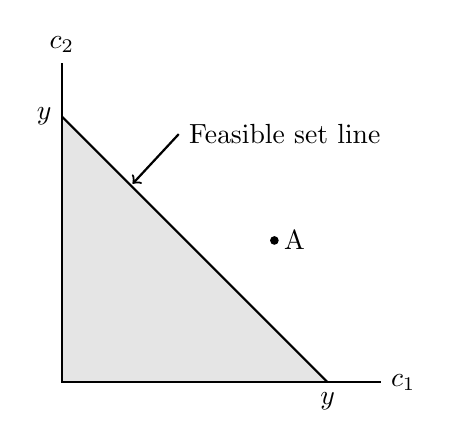
\begin{tikzpicture}[scale=0.45]
				\draw [fill=gray!20] (0,0) -- (0,7.5) -- (7.5,0);
				\draw [thick] (0,7.5) node [left]{\( y \)} to (7.5,0) node [below]{\( y \)};
				\draw [thick] (0,9) node[above]{\(c_2\)} -- (0,0) -- (9,0) node[right]{\(c_1\)};
				\filldraw [black] (6,4) circle (3pt) node[right]{A};
				\draw [thick, <-] (2,5.6) -- (3.3,7) node[right, align=left]{Feasible set line};
			\end{tikzpicture}
			\caption{The feasible set}
		\end{marginfigure}
		\item Within the feasible set, which allocation would the planner choose? The combination of \( (c_1, c_2) \) that maximizes an individual's utility.
		\item The golden rule allocation is the allocation within the feasible set that maximizes the utility of future generations. It occurs at the unique point of tangency between the feasible set line and an indifference curve
		\item Does the golden rule allocation maximize the utility of the initial old?
		\item Point A:\@ the golden rule allocation; Point E:\@ max utility of the initial old.
	\end{itemize}
	\begin{marginfigure}
		\centering
		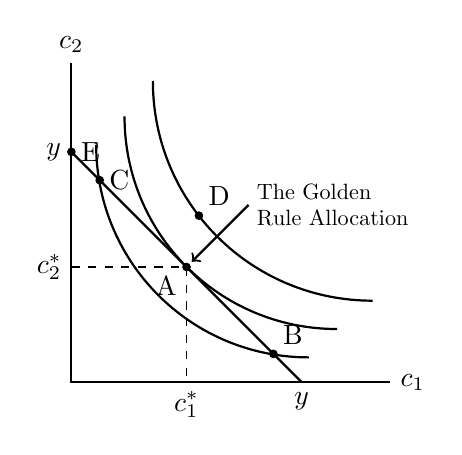
\begin{tikzpicture}[scale=0.45]
			\draw [thick] (0,6.5) node [left]{\( y \)} to (6.5,0) node [below]{\( y \)};
			\draw [thick] (0,9) node[above]{\(c_2\)} -- (0,0) -- (9,0) node[right]{\(c_1\)};
			\draw [dashed] (0,3.25) node[left]{\(c_2^*\)} -- (3.25,3.25) -- (3.25,0) node[below]{\(c_1^*\)};
			\filldraw [black] (3.25,3.25) circle (3pt) node[below left]{A};
			\filldraw [black] (5.7,0.8) circle (3pt) node[above right]{B};
			\filldraw [black] (0.8,5.7) circle (3pt) node[right]{C};
			\filldraw [black] (3.6,4.7) circle (3pt) node[above right]{D};
			\filldraw [black] (0,6.5) circle (3pt) node[right]{E};
			\draw [thick, <-] (3.4,3.4) -- (5,5) node[right, align=left,scale=0.8]{The Golden \\ Rule Allocation};
			\draw [thick] (1.5,7.5) to [out=-90,in=180] (7.5,1.5);
			\draw [thick] (2.3,8.5) to [out=-90,in=180] (8.5,2.3);
			\draw [thick] (0.7,6.7) to [out=-90,in=180] (6.7,0.7);
		\end{tikzpicture}
		\caption{Golden Rule allocation}
	\end{marginfigure}
\subsection{Decentralised Solutions: a Competitive Equilibrium without Money}
	\begin{itemize}
		\item To achieve the golden rule allocation, the planner needs to redistribute \( c_2^* \) units of goods from each young to each old in every period.
		\item Strong assumptions about the power of central planners.
		\item When individuals trade among themselves \( \rightarrow \) a competitive equilibrium.
		\begin{itemize}
			\item Individuals maximise their own utilities.
			\item Individuals are price takers.
			\item Markets clear.
		\end{itemize}
	\item No trade can occur in this economy \( \rightarrow \) autarkic allocation: individuals have no economic interaction with others.
	\begin{itemize}
		\item Lack of double coincidence of wants: the old would like to have some goods from the young, but they have nothing that the young want.
		\item No record-keeping or credit.
	\end{itemize}
	\item Each individual's consumption: \( c_1 = y, c_2 = 0. \) (Goods are non-storable!)
	\item Utility is low: both the future generations and the initial old are \textbf{worse off} than \textbf{almost} any other feasible consumption bundle.
	\end{itemize}
	\begin{marginfigure}
		\centering
		\begin{tikzpicture}[scale=0.45]
			\draw [thick] (0,6.5) node [above right]{C} to (6.5,0) node [above right]{B} node [below]{\( y \)};
			\draw [thick] (0,9) node[above]{\(c_2\)} -- (0,0) -- (9,0) node[right]{\(c_1\)};
			\filldraw [black] (3.25,3.25) circle (3pt) node[above right]{A};
		\end{tikzpicture}
		\caption{Decentralised solution}
	\end{marginfigure}
\subsection{Decentralised Solutions: a Monetary Equilibrium}
	\begin{itemize}
		\item How can the economy achieve a better allocation than the autarkic allocation?
		\item One way to allow some trading opportunities is to introduce \textbf{money}.
		\item Fiat money:
		\begin{itemize}
			\item produced by the government (almost) costlessly; \item cannot be counterfeited;
			\item portable;
			\item storable.
		\end{itemize}
		\item \textbf{A monetary equilibrium} is a competitive equilibrium in which there is a \textbf{valued} supply of fiat money.\@ that is, the fiat money can be traded for consumption good.
		\item For fiat money to have value, 2 conditions must be satisfied.
		\begin{itemize}
			\item supply of money must be limited.
			\item impossible (or very costly) to counterfeit.
		\end{itemize}
	\end{itemize}
	\subsubsection{Demand for Money}
	\begin{itemize}
		\item There is a fixed stock of money: \( M \) units.
		\item Each of the initial old is endowed with \( M/N_0 \) units money.
		\item Are there potential trade opportunities?
		\begin{itemize}
			\item At \( t = 1 \), the initial old have money and the young (newborn) have goods. Would they trade? Yes.
			\item At \( t = 2 \), the old (who were young at \( t = 1 \)) have money and the young (newborn) have goods. Would they trade? Yes.
			\item At \( t = 3,4, \dots, \) the old in each period always have some money and the young always have goods.
			\item Now each individual can consume in both periods of life.
		\end{itemize}
		\item  Consider an individual who is born at time \( t \).
		\begin{itemize}
			\item \( c_{1,t} \): consumption when young;
			\item \( c_{2,t+1} \): consumption when old;
			\item  \( m_t \): the number of dollars acquired when young (by giving up some of the endowed consumption good);
			\item \( v_t \): the value of money, which implies the price level \( p_t = \frac{1}{v_t} \)
		\end{itemize}
		\item The individual's budget constraint in the first period of life
		\[
			c_{1,t} + v_t m_t \leq y
		\]
		\item The individual's budget constraint in the second period of life
		\[
			c_{2,t+1} \leq v_{t+1}m_t
		\]
		\item The individual's life-time budget constraint
		\[
			c_{1,t} + \left(\frac{v_t}{v_{t+1}}\right) c_{2,t+1} \leq y.
		\]
		\begin{itemize}
			\item \( \left(\frac{v_t}{v_{t+1}}\right) \): the real return of money
		\end{itemize}
	\item Graphically, we depict the budget set
	\item Within the budget set, point A maximises an individual's utility.
	\end{itemize}
	\begin{marginfigure}
		\centering
		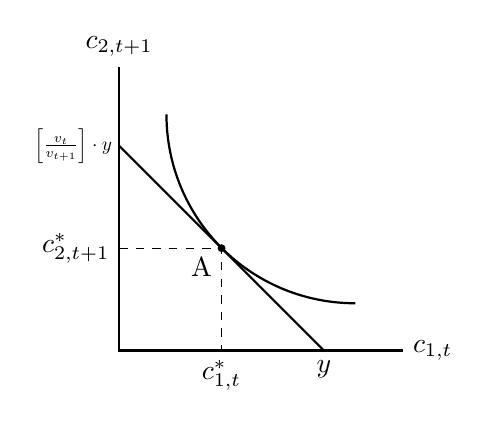
\begin{tikzpicture}[scale=0.4]
			\draw [thick] (0,6.5) node [left,scale=0.7]{\( \left[\frac{v_t}{v_{t+1}}\right] \cdot y \)} to (6.5,0) node [below]{\( y \)};
			\draw [thick] (0,9) node[above]{\(c_{2,t+1}\)} -- (0,0) -- (9,0) node[right]{\(c_{1,t}\)};
			\draw [dashed] (0,3.25) node[left]{\(c_{2,t+1}^*\)} -- (3.25,3.25) -- (3.25,0) node[below]{\(c_{1,t}^*\)};
			\filldraw [black] (3.25,3.25) circle (3pt) node[below left]{A};
			\draw [thick] (1.5,7.5) to [out=-90,in=180] (7.5,1.5);
		\end{tikzpicture}
		\caption{Demand for money}
	\end{marginfigure}
	\subsubsection{A Monetary Equilibrium}
	\begin{itemize}
		\item It remains to find \( \frac{v_{t+1}}{v_t} \). Recall that in any competitive market, the price (or value) of an object is determined as the price at which the supply of the object equals its demand.
		\begin{itemize}
			\item demand for money at time \( t \)
			\[
				N_t(y-c_{1,t});
			\]
			\item supply of money at time \( t \)
			\[
				v_t M_t;
			\]
			\item \( v_t \) is determined through
			\[
				N_t (y-c_{t,1}) = v_t M_t \rightarrow v_t=\frac{N_t(y-c_{1,t})}{M_t}
			\]
		\end{itemize}
		\item From \( v_t \) and \( v_{t+1} \), we can find
		\[
			\frac{v_{t+1}}{v_t} = \frac{\frac{N_{t+1}(y-c_1)}{M_{t+1}}}{\frac{N_t(y-c_1)}{M_t}} = \frac{\frac{N_{t+1}}{M_{t+1}}}{\frac{N_t}{M_t}}
		\]
		\item Let's further simplify our economy: suppose we focus on
		\begin{itemize}
			\item stationary allocations where \( c_{1,t} = c_1 \) and \( c_{2,t+1} = c_2 \); 
			\item a constant population where \( N_t = N \);
			\item a constant money supply where \( M_t = M \).
		\end{itemize}
		for all \( t \)
		\item Now, we have
		\[
			\frac{v_{t+1}}{v_t} = 1 \text{ or } v_{t+1} = v_t.
		\]
		The value of money is constant.
	\end{itemize}
	\begin{marginfigure}
		\centering
		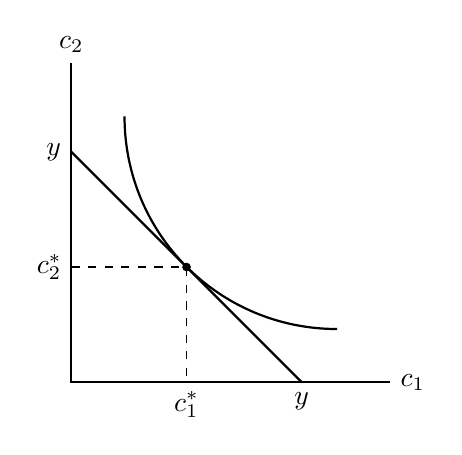
\begin{tikzpicture}[scale=0.45]
			\draw [thick] (0,6.5) node [left]{\( y \)} to (6.5,0) node [below]{\( y \)};
			\draw [thick] (0,9) node[above]{\(c_2\)} -- (0,0) -- (9,0) node[right]{\(c_1\)};
			\draw [dashed] (0,3.25) node[left]{\(c_2^*\)} -- (3.25,3.25) -- (3.25,0) node[below]{\(c_1^*\)};
			\filldraw [black] (3.25,3.25) circle (3pt);
			\draw [thick] (1.5,7.5) to [out=-90,in=180] (7.5,1.5);
		\end{tikzpicture}
	\end{marginfigure}
	\begin{itemize}
		\item Quantity theory of money: the price level is proportional to the quantity of money in the economy. In our economy, the price level is
		\[
			p = \frac{1}{v} = \frac{M}{N(y-c_1)}.
		\]
		\item Neutrality of money: the nominal size (measured in dollars) of the stock of money \( M \) has no effect on the real (measured in goods) values of consumption \( (c_1, c_2) \) and real money demand \( y - c_1 \).
	\end{itemize}
	\begin{table}[h]\centering
		\begin{tabular}{|c|c|}
			\hline
			golden rule & monetary equilbrium \\ \hline
			\begin{tabular}[c]{@{}c@{}}max utility\\ subject to the \textit{resource constraint}\end{tabular} & \begin{tabular}[c]{@{}c@{}}max utility \\ subject to the \textit{budget constraint}\end{tabular} \\ \hline
			resource constraint: \( c_1 + c_2 \leq y \) & budget constraint: \( c_1 + c_2 \leq y \) \\ \hline
			\multicolumn{2}{|c|}{golden rule = monetary equilibrium} \\ \hline
		\end{tabular}
	\end{table}
	\begin{itemize}
		\item Compared to competitive equilibrium without money, the introduction of money allows all future generations to achieve the golden rule allocation. It also benefits the initial old, whose consumption
		increases from 0 to \( c_2^* \).
	\end{itemize}
\subsection{A Growing Economy}
	\begin{itemize}
		\item So far we have learned that the introduction of money opens up trade opportunities and monetary equilibrium coincides with the golden rule allocation. We have assumed \textbf{a constant money supply} and \textbf{a constant population}.
		\item Suppose that \( N_t = nN_{t-1} \) where \( n > 1 \). How does a growing population affect the golden rule allocation and the monetary equilibrium?
		\item Golden rule allocation: the planner maximises an individual's utility subject to the resource constraint
		\[
			N_t c_1 + N_{t-1} c_2 \leq N_t y \rightarrow c_1 + \frac{1}{n} c_2 \leq y
		\]
	\end{itemize}
	\begin{marginfigure}
	\centering
	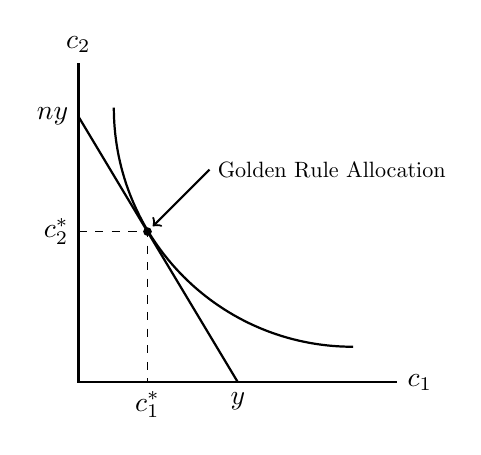
\begin{tikzpicture}[scale=0.45]
		\draw [thick] (0,7.5) node [left]{\( ny \)} to (4.5,0) node [below]{\( y \)};
		\draw [thick] (0,9) node[above]{\(c_2\)} -- (0,0) -- (9,0) node[right]{\(c_1\)};
		\draw [dashed] (0,4.25) node[left]{\(c_2^*\)} -- (1.95,4.25) -- (1.95,0) node[below]{\(c_1^*\)};
		\filldraw [black] (1.95,4.25) circle (3pt);
		\draw [thick] (1,7.75) to [out=-90,in=180] (7.75,1);
		\draw [thick, <-] (2.1,4.4) -- (3.7,6) node[right, align=left,scale=0.8]{Golden Rule Allocation};
	\end{tikzpicture}
	\caption{Golden rule allocation in a growing economy}
	\end{marginfigure}
	\begin{itemize}
		\item A Monetary equilibrium: the individual maximises his own utility subject to the life-time budget constraint
		\[
			c_1 + \left( \frac{v_t}{v_{t+1}} \right) c_2 \leq y.
		\]
		Recall that
		\[
			v_t = \frac{N_t (y-c_{t,1})}{M} \rightarrow \frac{v_{t+1}}{v_t} = \frac{N_{t+1}}{N_t} = n
		\]
		When the population is growing, the value of money is also growing at the same speed. Therefore, the budget constraint simplifies to
		\[
			c_1 + \frac{1}{n} c_2 \leq y.
		\]
		\item The budget constraint is identical to the resource constraint. So the monetary equilibrium coincides with the golden rule allocation. Again, the introduction of money helps the economy achieve the best possible allocation!
	\end{itemize}
\section{Inflation}
\subsection{Measuring Money}
	\begin{itemize}
		\item The definition of money as anything that is generally accepted in payments for goods and services does not tell us how we should measure money.
		\item Which assets shall we include when we measure money? Each country's central bank provides precise definitions.
		\item In Australia, the Reserve Bank of Australia (RBA) is responsible for monetary policy.
		\item RBA's definition of monetary aggregates:
		\begin{itemize}
			\item M0 or currency: notes and coins held by the private non-bank sector;
			\item M1: currency + current deposits with banks;
			\item M3: M1 + all other deposits at banks;
			\item Broad money: M3 + other borrowings from private sector by AFIs.
		\end{itemize}
		\item In general, currency < M1 < M3 < broad money.
	\end{itemize}
\subsection{Introduction}
	\begin{itemize}
		\item In our simple model of money, money supply is constant. From data on monetary aggregates, money supply seems to grow over time.
		\item The supply of fiat money is usually controlled by the central bank. Printing new money is an important way to finance government spending needs.
		\item In this section, we will examine
		\begin{itemize}
			\item the consequences of increasing money supply;
			\item the link between government spending and inflation;
			\item seigniorage: theory and evidence.
		\end{itemize}
	\end{itemize}
\subsection{Some Evidence}
	\begin{itemize}
		\item Money growth is the main determinant of inflation.
		\item A few examples of extraordinarily high inflation rates -- hyperinflations:
		\begin{itemize}
			\item Germany in 1923: inflation hits \( 3.25 \times 10^6 \) percent per month \( \rightarrow \) prices double every two days;
			\item Greece between 1941 and 1944:\@ inflation hits \( 8.55 \times 10^9 \) percent per month \( \rightarrow \) prices double every 28 hours;
			\item Yugoslavia between Oct 1993 and Jan 1994: inflation hits \( 5 \times 10^{15} \) percent per month \( \rightarrow \) prices double every 16 hours;
			\item Hungary after the end of WWII:\@ inflation peaks at \( 4.19 \times 10^{16} \) percent  per month \( \rightarrow \) prices double every 15 hours;
		\end{itemize}
		\item There could also be deflation. Examples:
		\begin{itemize}
			\item United States from 1930 to 1933;
			\item Hong Kong from late 1997 to 2004;
			\item Japan in the early 1990s.
		\end{itemize}
		\item To understand the causes and consequences of changing money growth rate, we will develop a theory.
	\end{itemize}
\subsection{A Growing Money Supply: New Money to the Public}
	\begin{itemize}
		\item Consider the OLG economy that we developed so far. Suppose that money supply grows at a rate \( z \):
		\[
			M_t = zM_{t-1}
		\]
		\item The amount of new money introduced into the economy in period \( t \) is:
		\[
			M_t - M_{t-1} = M_t - \frac{M_t}{z} = \left( 1-\frac{1}{z} \right) M_t
		\]
		\item New money is introduced into the economy by means of \textit{lump-sum} transfers to each \textbf{old} individual in every period \( t \) worth \( a_t \) units of consumption goods.
		\item To find the value of \( a_t \) in aggregate the government budget constraint is:
		\[
			N_{t-1}a_t = \left( 1-\frac{1}{z} \right) v_t M_t
		\]
		\[
			\Rightarrow a_t = \frac{\left( 1 - \frac{1}{z}\right) v_t M_t}{N_{t-1}}
		\]
	\end{itemize}
\subsubsection{A Monetary Equilibrium}
	\begin{itemize}
		\item Budget constraints:
		\begin{itemize}
			\item first period of life:
			\[
				c_{1,t} + v_t m_t \leq y;
			\]
			\item second period of life:
			\[
				c_{2,t+1} \leq v_{t+1} m_t + a_{t+1};
			\]
			\item lifetime budget constraint
			\[
				c_{1,t} + \frac{v_t}{v_{t+1}} c_{2,t+1} \leq y + \frac{v_t}{v_{t+1}} a_{t+1}.
			\]
		\end{itemize}
		\item What is the value of \( \frac{v_{t+1}}{v_t} \)? As before, we first solve for \( v_t \) from money market clearing condition.
		\[
		v_t M_t = N_t (y-c_{1,t}) \rightarrow v_t = \frac{N_t (y-c_{1,t})}{M_t}
		\]
		\item As usual, we focus on stationary allocations. \textbf{Assume for now that the population is constant.}
		\item The value of money is then
		\[
			v_t = \frac{N (y-c_1)}{M_t}.
		\]
		\item It follows that
		\[
			\frac{v_{t+1}}{v_t} = \frac{\frac{N_{t+1} (y-c_1)}{M_{t+1}}}{\frac{N_t (y-c_1)}{M_t}} = \frac{M_t}{M_{t+1}} = \frac{M_t}{zM_t} = \frac{1}{z}
		\]
		\item Furthermore, the price level
		\[
			\frac{p_{t+1}}{p_t} = \frac{\frac{1}{v_{t+1}}}{\frac{1}{v_t}} = \frac{v_t}{v_{t+1}} = z.
		\]
		\item When money supply is growing at a rate z, the price level increases at a rate \( z \). \textbf{Quantity Theory of Money!}
		\item An individual's budget constraint simplifies to
		\[
			c_1 + zc_2 \leq y + za
		\]
	\end{itemize}
	\begin{figure}[H]
		\centering
		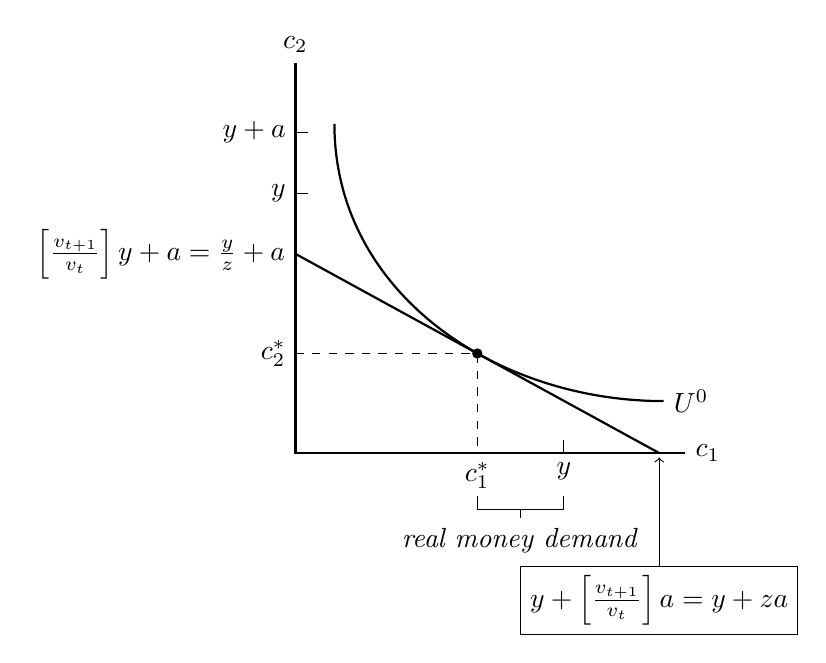
\begin{tikzpicture}[scale=0.55]
			\draw [thick] (0,4.6) node [left]{\( \left[ \frac{v_{t+1}}{v_t}  \right] y + a = \frac{y}{z} + a \)} to (8.4,0);
			\draw [->] (8.4,-2.6) node [draw, below] {\( y + \left[ \frac{v_{t+1}}{v_t} \right] a = y + za \)} -- (8.4,-0.1);
			\draw [thick] (0,9) node[above]{\(c_2\)} -- (0,0) -- (9,0) node[right]{\(c_1\)};
			\draw [dashed] (0,2.3) node[left]{\(c_2^*\)} -- (4.2,2.3) -- (4.2,0) node [below] {\(c_1^*\)};
			\draw (0,6) node [left] {\(y\)} -- (0.3,6);
			\draw (0,7.4) node [left] {\(y+a\)} -- (0.3,7.4);
			\draw (6.2,0) node [below] {\(y\)} -- (6.2,0.3);
			\draw (4.2,-1) -- (4.2,-1.3) -- (6.2,-1.3) -- (6.2,-1);
			\draw (5.2,-1.3) -- (5.2,-1.5) node [below] {\textit{real money demand}};
			\filldraw [black] (4.2,2.3) circle (3pt);
			\draw [thick] (8.5,1.2) node [right]{\( U^0 \)} to [out=-180,in=-90] (0.9,7.6) ;
		\end{tikzpicture}
	\end{figure}
	\begin{itemize}
		\item The solution \( (c_1^* c_2^*) \) are functions of \( (z,y,a) \). To close the model, we need to find the value of \( a \). Recall that from the government budget constraint
		\[
			N_{t-1} a_t = \left( 1 - \frac{1}{z} \right) v_t M_t. 
		\]
		\( a \) is solved from
		\[
			a = \frac{\left( 1 - \frac{1}{z}\right) v_t M_t}{N} = \frac{\left( 1 - \frac{1}{z}\right) \frac{N (y-c_1)}{M_t} M_t}{N} = \left( 1 - \frac{1}{z} \right) (y - c_1^*).
		\]
		\item In a monetary equilibrium, \( (c_1^*,c_2^*) \) maximises an individual utility subject to the lifetime budget constraint is \textbf{satisfied} in every period.
		\item An example: if \( u(c_1,c_2) = c_1c_2, \) an individual
		\[
			\max_{c_1,c_2} c_1c_2 \quad \text{ subject to } c_1 + zc_2 \leq y + za
		\]
		We have
		\[
			c_1 = \frac{y + za}{2} \text{ and } c_2 = \frac{y + za}{2z}
		\]
		We can also find \( a \) by solving
		\[
			a = \left( 1 - \frac{1}{z} \right) \left( y - \frac{y + za}{2}\right) \rightarrow a = \frac{y \left( 1 - \frac{1}{z} \right) }{1+z} 
		\]
		Substituting \( a \) into \( (c_1,c_2) \), we have
		\[
			c_1 = \frac{yz}{1+z} \text{ and } c_2 = \frac{y}{1+z}.
		\]
	\end{itemize}
\subsubsection{Is the Monetary Equilibrium Efficient?}
	\begin{itemize}
		\item Consider the model with a constant population and a growing money supply, \( M_t = zM_{t-1} \)
		\item An individual's budget constraint
		\[
		c_1 + zc_2 \leq y + za
		\]
		\item The golden allocation: a planner maximises and individual's utility subject to the resource constraint.
		\[
			Nc_1 + Nc_2 \leq Ny \:\rightarrow\: c_1 +c_2 \leq y
		\]
	\end{itemize}
	\begin{figure}[H]
		\centering
		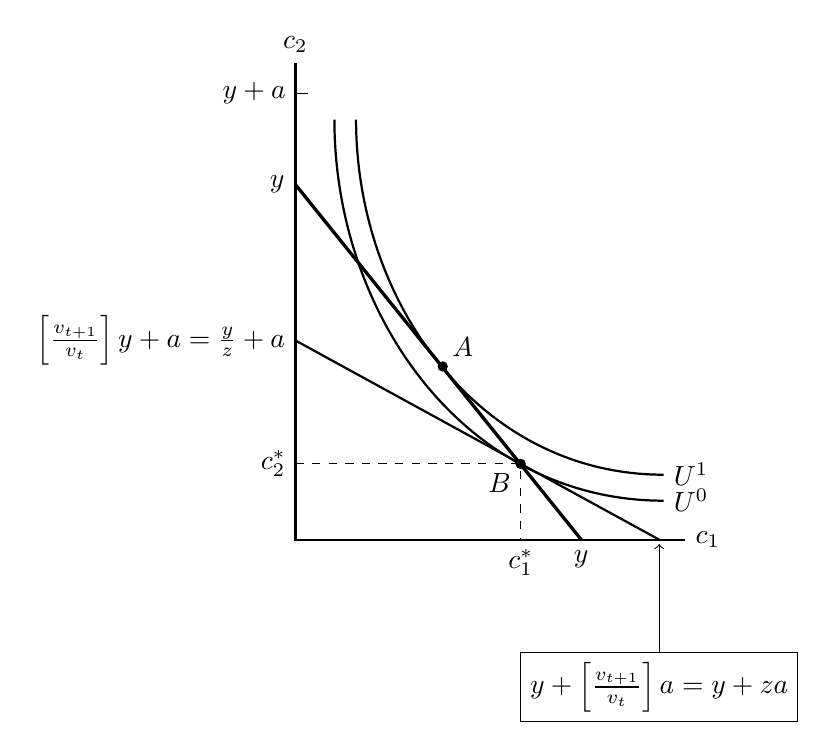
\begin{tikzpicture}[scale=0.55]
			\draw [thick] (0,4.6) node [left]{\( \left[ \frac{v_{t+1}}{v_t}  \right] y + a = \frac{y}{z} + a \)} to (8.4,0);
			\draw [->] (8.4,-2.6) node [draw, below] {\( y + \left[ \frac{v_{t+1}}{v_t} \right] a = y + za \)} -- (8.4,-0.1);
			\draw [thick] (0,11) node[above]{\(c_2\)} -- (0,0) -- (9,0) node[right]{\(c_1\)};
			\draw [dashed] (0,1.75) node[left]{\(c_2^*\)} -- (5.2,1.75) -- (5.2,0) node [below] {\(c_1^*\)};
			\draw [very thick] (0,8.2) node [left] {\(y\)} -- (6.6,0) node [below] {\(y\)};
			\draw (0,10.3) node [left] {\(y+a\)} -- (0.3,10.3);
			\draw [thick] (8.5,0.9) node [right]{\( U^0 \)} to [out=-180,in=-90] (0.9,9.7);
			\draw [thick] (8.5,1.5) node [right]{\( U^1 \)} to [out=-180,in=-90] (1.4,9.7);
			\filldraw [black] (3.4,4) circle (3pt) node [above right] {\( A \)};
			\filldraw [black] (5.2,1.75) circle (3pt) node [below left] {\( B \)};
		\end{tikzpicture}
	\end{figure}
	\begin{itemize}
		\item Compare monetary equilibrium allocation at point \( B \) with the golden rule allocation at point \( A \).
		\item Monetary equilibrium at point \( B \): intersection of the budget constraint and the resource constraint.
		\item With a growing money supply, the allocation in a monetary equilibrium is not the golden rule allocation.
		\begin{itemize}
			\item  Young consume more \( \rightarrow \) noncash goods.
			\item  Old consume less \( \rightarrow \) cash goods.
		\end{itemize}
		\item In a monetary equilibrium, all future generations are worse off: utility at point \( B \) is lower than utility at point \( A \). The initial old are also worse off.
	\end{itemize}
\subsubsection{Cost of Inflation}
	\begin{itemize}
		\item In general, effects of inflation:
		\begin{center}
			people are less willing to hold money and economise the use of money,
			\[\downarrow\]
			transactions that are conducted using money are adversely affected,
			\[\downarrow\]
			violates ``smooth consumption'' assumption
			\[\downarrow\]
			welfare fall.
		\end{center}
		\item Inflation is effectively a tax
	\end{itemize}
\subsubsection{A Growing Population}
	\begin{itemize}
		\item Suppose that population grows such that \( N_t = n N_{t-1} \)
		\item Budget constraints:
		\begin{itemize}
			\item first period budget constraint:
			\[
				c_1 + v_t m_t \leq y;
			\]
			\item second period budget constraint:
			\[
				c_2 \leq v_{t+1} m_t + a;
			\]
			\item lifetime budget constraint
			\[
				c_1 + \frac{v_t}{v_{t+1}} c_2 \leq y + \frac{v_t}{v_{t+1}} a.
			\]
		\end{itemize}
	\item Value of money \( v_t \):
	\[
		N_t (y-c_1) = v_tM_t \rightarrow v_t = \frac{N_t (y-c_1)}{M_t}
	\]
	\item Money's rate of return \(\frac{v_t+1}{v_t}\):
	\[
		\frac{v_{t+1}}{v_t}  = \frac{\frac{N_{t+1} (y-c_1)}{M_{t+1}}}{\frac{N_t (y-c_1)}{M_t}} = \frac{N_t}{N_{t+1}} \frac{M_t}{M_{t+1}} = \frac{n}{z}
	\]
	The value of money may increase or decrease over time depending on the values of \( n \) and \( z \).
	\item An individual's lifetime budget constraint simplifies to
	\[
		c_1 + \frac{z}{n} c_2 \leq y + \frac{z}{n} \cdot a.
	\]
	\item Graphically, we depict the budget constraint and the allocation \( B \) that is chosen in a monetary equilibrium. Allocation \( A \) is the golden rule allocation.
	\end{itemize}
	\begin{figure}[H]
		\centering
		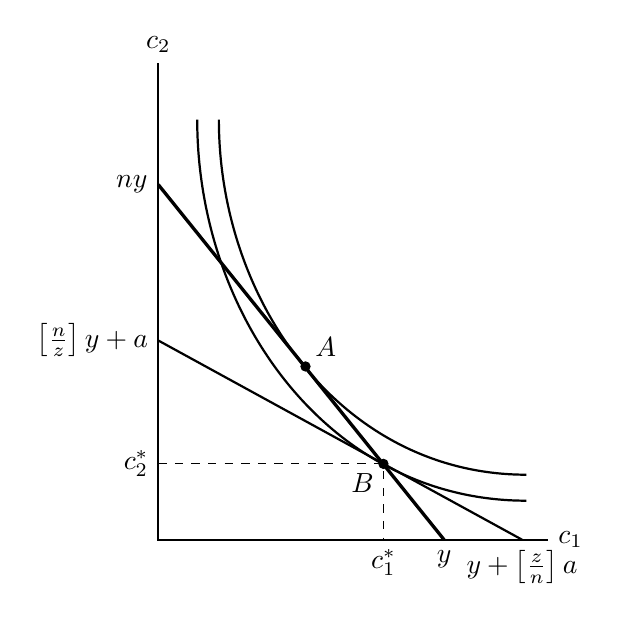
\begin{tikzpicture}[scale=0.55]
			\draw [thick] (0,4.6) node [left]{\( \left[ \frac{n}{z} \right] y + a \)} to (8.4,0) node [below] {\( y + \left[ \frac{z}{n} \right] a \)};
			\draw [thick] (0,11) node[above]{\(c_2\)} -- (0,0) -- (9,0) node[right]{\(c_1\)};
			\draw [dashed] (0,1.75) node[left]{\(c_2^*\)} -- (5.2,1.75) -- (5.2,0) node [below] {\(c_1^*\)};
			\draw [very thick] (0,8.2) node [left] {\(ny\)} -- (6.6,0) node [below] {\(y\)};
			\draw [thick] (8.5,0.9) to [out=-180,in=-90] (0.9,9.7);
			\draw [thick] (8.5,1.5) to [out=-180,in=-90] (1.4,9.7);
			\filldraw [black] (3.4,4) circle (3pt) node [above right] {\( A \)};
			\filldraw [black] (5.2,1.75) circle (3pt) node [below left] {\( B \)};
		\end{tikzpicture}
	\end{figure}
	\begin{itemize}
		\item Golden rule allocation: a planner's resource constraint
		\[
			N_tc_1 + N_{t-1} c_2 \leq N_t y \quad \rightarrow \quad c_1 \frac{1}{n} c_2 \leq y
		\]
		\item The resource constraint is different from the individual's budget constraint. The allocation in a monetary equilibrium is not the golden rule allocation. Again, the expansion of money supply makes individuals consume more when young and less when old. The overall utility is lower than the utility at the golden rule allocation.
		\item What is the optimal growth rate of money supply in an economy with a growing population? To make the individual's  budget constraint identical to the resource constraint, it requires
		\[
			\frac{v_{t+1}}{v_t} = \frac{n}{z} = n
		\]
		It means that \( z = 1 \). A constant money supply allows the economy to achieve the golden rule allocation.
		\begin{itemize}
			\item Planner's resource constraint: if each young gives up 1 unit of consumption, the old can receives \( n \) units.
			\item Individual's budget constraint: if the young gives up 1 unit of consumption, he will receive \( n/z \) units when old.
			\item To convey the message that the economy can offer \( n \) units of goods to the old for each good not consumed by the young, the budget constraint has to be adjusted so that it coincides with the resource constraint.
			\item The value of money needs to increase at a rate \( n \). That is \( \frac{v_{t+1}}{v_t} = n \)
		\end{itemize}
	\end{itemize}
\subsubsection{Summary}
	\begin{itemize}
		\item So far, we have shown that when money supply grows at a rate \( z \) with \( z > 1 \), the allocation in a monetary equilibrium generally differs from the golden rule allocation.
		\item Inflation reduces individuals incentives to hold money and adversely affects transactions using money. As a result, inflation may reduce output and welfare.
		\item In our model, the optimal growth rate of money supply is \textbf{always} \( z = 1 \), no matter the population is constant or growing. That is, \textbf{a constant money supply is the best policy}.
	\end{itemize}
\subsection{A Growing Money Supply: New Money to Finance Government Purchases}
\subsubsection{A Monetary Equilibrium}
	\begin{itemize}
		\item Government needs to create revenue to finance various types of expenditures. The use of money creation as a revenue device is called \textbf{``seigniorage''}
		\item We focus on stationary allocations and a constant population.
		\item Suppose that money supply grows at a constant rate \( z: M_t = zM_{t-1} \)
		\begin{itemize}
			\item The amount of new money created in period \( t \) is
			\[
				M_t - M_{t-1} = M_t - \frac{1}{z} M_t = \left( 1 - \frac{1}{z} \right) M_t. 
			\]
			\item The amount of goods that the government can purchase in period \( t \) is
			\[
				G_t = v_t (M_t - M_{t-1}) = \left( 1 - \frac{1}{z} \right) v_t M_t.
			\]
			This is also the government budget constraint.
			\item Suppose that \( G_t \) does not affect an individual's consumption choice.
		\end{itemize}
		\item Budget constraints:
		\begin{itemize}
			\item first period budget constraint:
			\[
				c_1 + v_t m_t \leq y;
			\]
			\item second period budget constraint:
			\[
				c_2 \leq v_{t+1} m_t;
			\]
			\item lifetime budget constraint
			\[
				c_1 + \frac{v_t}{v_{t+1}} c_2 \leq y.
			\]
			\item Notice that in this model, \textbf{individuals do not receive government transfers}.
		\end{itemize}
		\item Money's rate of return \( \frac{v_{t+1}}{v_t} \):
		\begin{itemize}
			\item value of money \( v_t \) is determined when money market clears
			\[
				N (y-c_1) = v_t M_t \quad \rightarrow \quad v_t = \frac{N(y-c_1)}{M_t}
			\]
			\item money's rate of return
			\[
				\frac{v_t+1}{v_t}  = \frac{\frac{N_{t+1} (y-c_1)}{M_{t+1}}}{\frac{N_t (y-c_1)}{M_t}} = \frac{M_t}{M_{t+1}} = \frac{1}{z}
			\]
		\end{itemize}
	\item We simplify the individual's budget constraint to
	\[
		c_1 + zc_2 \leq y
	\]
	\item Graphically, we depict the budget constraint and add a typical indifference curve.
	\end{itemize}
	\begin{figure}[H]
		\centering
		\begin{tikzpicture}[scale=0.55]
			\draw [thick] (0,4.6) node [left]{\( \frac{y}{z} \)} to (8.4,0) node [below] {\( y \)};
			\draw [thick] (0,9) node[above]{\(c_2\)} -- (0,0) -- (9,0) node[right]{\(c_1\)};
			\draw [dashed] (0,2.3) node[left]{\(c_2^*\)} -- (4.2,2.3) -- (4.2,0) node [below] {\(c_1^*\)};
			\filldraw [black] (4.2,2.3) circle (3pt);
			\draw [thick] (8.5,1.2) to [out=-180,in=-90] (0.9,7.6);
		\end{tikzpicture}
	\end{figure}
	\begin{itemize}
		\item In a monetary equilibrium, the amount of goods that the government can purchase in period \( t \) can be found from
		\[
			G_t = \left( 1 - \frac{1}{z} \right) v_t M_t = \left( 1 - \frac{1}{z} \right) N (y-c_1).
		\]
		Notice that \( G_t \) is also stationary because \( G_t = G_{t+1} \) for any \( t \).
	\end{itemize}
\subsubsection{Golden Rule Allocation}
	\begin{itemize}
		\item To discuss the optimality of monetary equilibrium, we need to find the golden rule allocation.
		\item The planner's resource constraint
		\[
			Nc_1 = Nc_2 + G \leq Ny
		\]
		where \( G_t = G \) for stationary allocations. Divide both sides by \( N \) and let \( g \equiv \frac{G}{N} \). The resource constraint can be rewritten as
		\[
			c_1 + c_2 + g \leq y
		\]
		Notice that when the government uses new money to finance its own purchases, \( G \) or \( g \) is in the resource constraint. The government competes with individuals for resources.
		\item Graphically, we depict the resource constraint and add a typical indifference curve.
	\end{itemize}
	\begin{figure}[H]
		\centering
		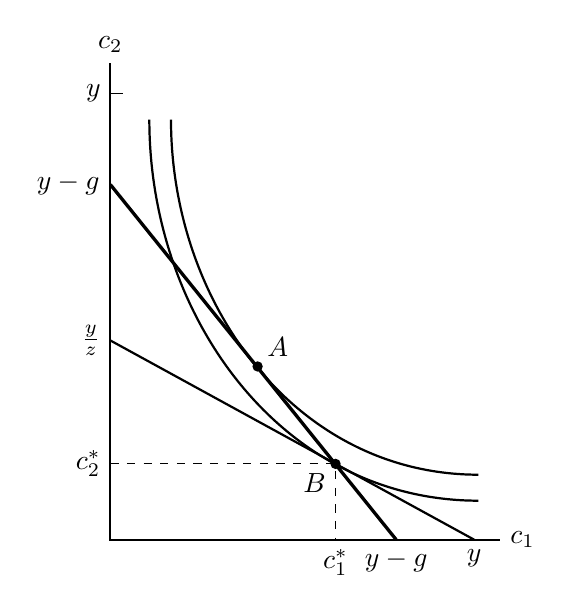
\begin{tikzpicture}[scale=0.55]
			\draw [thick] (0,4.6) node [left]{\( \frac{y}{z} \)} to (8.4,0) node [below] {\( y \)};
			\draw [thick] (0,11) node[above]{\(c_2\)} -- (0,0) -- (9,0) node[right]{\(c_1\)};
			\draw [dashed] (0,1.75) node[left]{\(c_2^*\)} -- (5.2,1.75) -- (5.2,0) node [below] {\(c_1^*\)};
			\draw [very thick] (0,8.2) node [left] {\(y - g\)} -- (6.6,0) node [below] {\(y - g\)};
			\draw (0,10.3) node [left] {\(y\)} -- (0.3,10.3);
			\draw [thick] (8.5,0.9) to [out=-180,in=-90] (0.9,9.7);
			\draw [thick] (8.5,1.5) to [out=-180,in=-90] (1.4,9.7);
			\filldraw [black] (3.4,4) circle (3pt) node [above right] {\( A \)};
			\filldraw [black] (5.2,1.75) circle (3pt) node [below left] {\( B \)};
		\end{tikzpicture}
	\end{figure}
	\begin{itemize}
		\item We compare monetary equilibrium at point \( B \) with the golden rule allocation at point \( A \).
		\item When the government prints new money to finance its own purchases, the allocation in a monetary equilibrium achieves a lower level of utility than the golden rule allocation.
		\item Inflation makes individuals trade less goods for money when young, which leads to
		\begin{itemize}
			\item higher consumption when young;
			\item lower consumption when old.
		\end{itemize}
		\item Note that in comparison with the golden rule allocation, inflation hurts all future generations, as well as the initial old because \( c_2^* \) is lower in a monetary equilibrium.
	\end{itemize}
\subsubsection{Inflation Tax v.s. Nondistorting Tax}
	\begin{itemize}
		\item Creating new money is one way to finance government purchases \( \rightarrow \) effectively an inflation tax. As we have shown, inflation leads to the monetary equilibrium allocation at point \( B \), which is inferior to the golden rule allocation at point \( A \).
		\item Given the need for the government to raise revenue, are there other ways to raise revenue and make the golden rule allocation attainable?
		\item Consider a \textbf{lump-sum tax}. Suppose that the government collects a  tax of \( \tau \) goods from each old individual in every period.
		\item Monetary equilibrium:
		\begin{itemize}
			\item first-period budget constraint
			\[
				c_1 + v_t m_t \leq y;
			\]
			\item second-period budget constraint
			\[
				c_2 \leq v_{t+1} m_t - \tau;
			\]
			\item lifetime budget constraint
			\[
				c_1 + \frac{v_t}{v_{t+1}} c_2 \leq y - \frac{v_t}{v_{t+1}} \tau.
			\]
		\end{itemize}
		\item How can the government choose the values of \( \frac{v_t}{v_{t+1}} \) and \( \tau \) so that
		\begin{itemize}
			\item monetary equilibrium can be the same as the golden rule allocation;
			\item the government can still finance its own purchases \( G \)?
		\end{itemize}
		\item The government can keep a constant money supply by imposing \( \tau = g \) In this case, we can verify \( \frac{v_t}{v_{t+1}} = 1 \) and the individual's budget constraint becomes
		\[
			c_1 + c_2 \leq y - g
		\]
		Now the budget constraint is identical to the planner's resource constraint. The allocation in a monetary equilibrium is the same as the golden rule allocation.
		\item Inflation tax (creating new money) and lump-sum taxes:
		\begin{itemize}
			\item inflation tax: inferior equilibrium allocation but easy to implement -- low cost
			\item lump-sum taxes: golden rule allocation but hard to implement in reality.
		\end{itemize}
		\item Money creation has been a popular means to raise government revenue.
	\end{itemize}
\subsubsection{Seigniorage: Theory and Evidence}
	\begin{itemize}
		\item The use of seigniorage as a source of government revenue varies from country to country and from time to time.
		\begin{itemize}
			\item For most developed countries during normal times: seigniorage contributes little to government revenue. For example, seigniorage in U.S. accounted for about 2\% of total government revenue and for about 0.3\% of gross national product from 1948 to 1989.
			\item For countries that experience high inflation episodes like Argentina, Chile and etc., seigniorage contributes significantly to government revenue. For example, seigniorage accounted for about 46\% of Argentinian government revenue and 6.2\% of gross national product from 1960 to 1975.
			\item An extreme case: Germany during its hyperinflation of the early 1920s. Seigniorage was about 10\% to 15\% of gross national product.
		\end{itemize}
		\item Can the government simply print enough money to finance any purchase without the bother of direct taxation?
		\begin{itemize}
			\item The government can print any amount of dollars.
			\item The value of those dollars may shrink as the supply of money increases.
			\item Seigniorage revenue in terms of real goods is limited by the real value of money.
		\end{itemize}
		\item To formally examine how seigniorage revenue depends on the speed of money creation, we revisit the government budget constraint
		\[
			G = (M_t - M_{t-1}) v_t = \underbrace{\left( 1- \frac{1}{z} \right) }_\text{tax rate} \underbrace{v_t M_t}_\text{tax base}
		\]
		\item There are two terms in \( G \).
		\begin{itemize}
			\item \( 1 - \frac{1}{z} \): \textit{tax rate} the fraction of the real value of the money stock that becomes government revenue;
				\begin{itemize}
					\item example: if \( z = 1.05 \), then \( 1 - 1/z = 1 - 1/1.05 = 0.0476 \).
				\end{itemize}
			\item \( v_t M_t \): \textit{tax base} -- the real value of the money stock (the value of the money stock in terms of goods).
		\end{itemize}
		\item When the government increases the speed of printing money by raising \( z \),
		\begin{itemize}
			\item the tax rate \( 1 - 1/z \) will increase;
			\item but what is the effect of z on the tax base \( v_t M_t \)?
		\end{itemize}
		\item Recall: from the money market clearing condition
		\[
			v_t M_t = N (y-c_1).
		\]
		\item We need to know how \( c_1 \) depends on z.
		\item Consider \( z^1 \) and \( z^2 \) where \( z^2 \) > \( z^1 \). How does \( c_1 \) respond to an increase in \( z \) from \( z^1 \) to \( z^2 \)?
		\begin{itemize}
			\item \( (c_1, c_2) \) in a monetary equilibrium is determined by the tangency point between the indifference curve and the budget constraint.
			\item The budget constraint in this economy is
			\[
				c_1 + zc_2 \leq y
			\]
			An increase in z would affect the individual's budget constraint.
		\end{itemize}
		\item Graphically, when \( z \) increases from \( z^1 \) to \( z^2 \), \( c_1 \) increases from \( c_1^1 \) to \( c_1^2 \)
	\end{itemize}
	\begin{figure}[H]
		\centering
		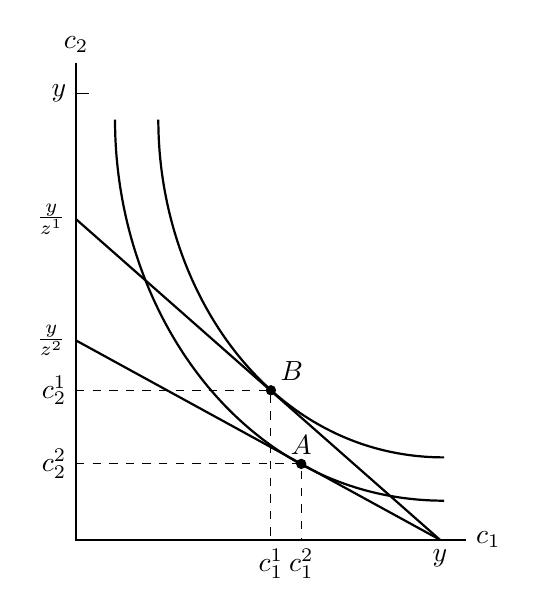
\begin{tikzpicture}[scale=0.55]
			\draw [thick] (0,4.6) node [left]{\( \frac{y}{z^2} \)} to (8.4,0) node [below] {\( y \)};
			\draw [thick] (0,7.4) node [left]{\( \frac{y}{z^1} \)} to (8.4,0);
			\draw [thick] (0,11) node[above]{\(c_2\)} -- (0,0) -- (9,0) node[right]{\(c_1\)};
			\draw (0,10.3) node [left] {\(y\)} -- (0.3,10.3);
			\draw [thick] (8.5,0.9) to [out=-180,in=-90] (0.9,9.7);
			\draw [thick] (8.5,1.9) to [out=-180,in=-90] (1.9,9.7);
			\filldraw [black] (4.5,3.45) circle (3pt) node [above right] {\( B \)};
			\draw [dashed] (0,3.45) node [left] {\( c_2^1 \)}-- (4.5,3.45) -- (4.5,0) node [below] {\( c_1^1 \)};
			\filldraw [black] (5.2,1.75) circle (3pt) node [above] {\( A \)};
			\draw [dashed] (0,1.75) node [left] {\( c_2^2 \)}-- (5.2,1.75) -- (5.2,0) node [below] {\( c_1^2 \)};
		\end{tikzpicture}
	\end{figure}
	\begin{itemize}
		\item When \( z \) increases, the inflation rate increases. Higher inflation induces young to trade less goods for money so that \( c_1 \) increases and \( c_2 \) decreases.
		\item Now, back to our money market clearing condition
		\[
			c_1 + zc_2 \leq y
		\]
		When \( c_1 \) increases, the aggregate demand for money in real terms \( N (y - c_1) \) decrease. Therefore, the aggregate supply of money in real terms \( v_t M_t \) also decrease. The tax base \( v_t M_t \) decreases.
		\item Economists have found evidence that higher inflation leads to lower real demand for money
		\item So far, we have found that when growth rate of money supply \( z \) increases,
		\begin{itemize}
			\item the tax rate \( 1-\frac{1}{z} \) increases;
			\item the tax base \( v_t M_t \) decreases;
		\end{itemize}
		\item Overall, seigniorage revenue
		\[
			G = \left( 1-\frac{1}{z} \right) v_t M_t = \left( 1-\frac{1}{z} \right) N(y - c_1),
		\]
		may or may not increase as \( z \) increases. The exact relationship between the seigniorage revenue \( G \) and the growth rate of money supply \( z \) depends on the utility function of individuals and anything else that affects the demand for money.
		\item The general shape of \( G \) as a function of \( z \) \textbf{resembles} the Laffer curve:
			\begin{itemize}
				\item at low growth rates of money supply, a higher growth rate leads to a higher level of seigniorage;
				\item at high growth rates of money supply, a higher growth rate leads to a lower level of seigniorage;
				\item there exists a growth rate of money supply that maximizes seigniorage.
			\end{itemize}
		\item The original Laffer curve describes the relationship between income tax rate and income tax revenue.
	\end{itemize}
	\begin{figure}[H] \centering
		\begin{tikzpicture}
			\begin{axis}[
				ylabel = {Real Seigniorage Level},
				axis on top,
				no markers,
				xmin = 1,
				xmax = 12,
				ticks=none,
				]
				\addplot+[black, smooth, no markers, domain=1:12] {20000*((1-(1/x))/(1+x))};
			\end{axis}
		\end{tikzpicture}
	\end{figure}
\section{Price Surprises}
\subsection{Introduction}
	\begin{itemize}
		\item The relationship between inflation and unemployment -- the Phillips curve.
		\item Cross country evidence on the relationship between inflation and output.
		\item We develop a theory to rationalise the empirical observations?
		\begin{itemize}
			\item \textbf{Unanticipated} changes in money supply. In previous sections, we consider \textbf{anticipated} increases in money supply.
			\item How do unanticipated fluctuations in money supply affect output?
			\item Can the government exploit such a relationship?
		\end{itemize}
		\item The Lucas (1972) model and the Lucas critique.
	\end{itemize}
\subsection{The Data}
\subsubsection{The Phillips Curve}
	\begin{itemize}
		\item The original Phillips curve suggests that there is a negative relationship between inflation and unemployment, or there is a positive relationship between inflation and output.
		\item Does it imply that there maybe an exploitable trade-off between inflation and unemployment? Can the government reduce unemployment and increase output by increasing inflation?
		\item In the following decades, many governments tried to use monetary policy to stimulate the economy. Suddenly, the Phillips curve, a stable relationship for more than a century, disappeared. Inflation occurs with no gains in output or employment.
	\end{itemize}
\subsubsection{Cross-country Comparisons}
	\begin{itemize}
		\item The Phillips curve is a \textbf{time series} correlation between inflation and unemployment in different periods of the same country.
		\item If we compare across countries, inflation rates are on average higher in countries with lower average real GDP growth rates. Note: its a \textbf{cross-section} comparison here.
		\item How can there exist seemingly contradictory correlations
		\begin{itemize}
			\item Time series of the same country: \textbf{-ve} correlation between inflation and unemployment, that is, \textbf{+ve} correlation between inflation and output.
			Cross-country comparisons: \textbf{-ve} correlation between inflation and output.
		\end{itemize}
	\end{itemize}
\subsection{The Lucas Model}
\subsubsection{Basic Environment}
	\begin{itemize}
		\item Consider the standard OLG model with money. Now assume that individuals live on two spatially separated islands.
		\item \( N_t \) individuals are born in each period. \( N_t \) is constant. In each period,
		\begin{itemize}
			\item half of the old live on each of the islands;
			\item 1/3 of the young live on one island and 2/3 live on the other island;
			\item the allocation of the young and the old is random.
			\begin{itemize}
				\item the old are randomly distributed across the two islands, regardless of where they lived when young
				\item in any single period, each island has an equal chance of having the large population of young.
			\end{itemize}
			\item Money supply grows at a rate \( z_t \) in period \( t , M_t = z_t M_{t-1} \). The new money is distributed to each old person as a lump-sum transfer in
				every period t worth at units of the consumption good.
		\end{itemize}
		\item Money supply grows at a rate \( z_t \) in period \( t \), \( M_t = z_t M_{t-1} \). The new money is distributed to each \textbf{old} person as a lump-sum transfer in every period t worth at units of the consumption good.
		\[
			a_t = \left( 1 - \frac{1}{z_t} \right) \frac{v_t M_t}{N}
		\]
		\item Informational assumptions: in any period,
		\begin{itemize}
			\item the young cannot observe the number of young individuals on their island;
			\item the young cannot observe the size of the transfers to the old;
			\item the nominal stock of money supply is known with a delay of one period; e.g., in period \( t \), individuals know \( M_{t-1} \), but not \( M_t \);
			\item the price of goods on an island is observed but only by the individuals on that island;
			\item no communication between islands within a period.
		\end{itemize}
		\item We assume that individuals are rational.
		\begin{itemize}
			\item They may not have complete information, but they can infer whatever they can from the information they have and they make the most correct inference possible given the explicitly specified limits on what they can observe.
			\item The assumption of ``rational expectation'', first introduced by Muth (1961): people understand the probabilities of outcomes important to their welfare.
			\item In our model, individuals do not observe \( z_t \) and the population of the young on each island, but they know the prices. They know 1/3 of the young are on one island and the rest 2/3 are on the other island. They will try to infer \( z_t \) and the distribution of the young population.
		\end{itemize}
		\item A reinterpretation of an individual's problem.
		\begin{itemize}
			\item \( y \): individuals are endowed when young with y units of time (instead of goods): think of \( y \) as 24 hours;
			\item \( c_1 \): consumption of \textbf{leisure} (instead of consumption of goods); \( y - c_1 \) is spent working;
			\item \( c_2 \): consumption of goods;
			\item \( I = y - c_1 \): labour supply by the individual when young; \( l_t^i = l(p_t^i) \): the choice of labour by an individual born in period \( t \) for a given price of goods, \( p_t^i \) on island \( i \);
			\item production function: 1 unit of \( l \) can be used to produce 1 unit of the consumption goods
		\end{itemize}
		\item Consumption
	\end{itemize}
	\begin{table}[h]\centering
		\begin{tabular}{|c|c|c|c|c|c|}
			\hline
			Generation & t=1 & t=2 & t=3 & t=4 & \( \longrightarrow \) \\ \hline
			0 & \( c_2 \) &  &  &  &  \\ \hline
			1 & \( c_1 \) & \( c_2 \) &  &  &  \\ \hline
			2 &  & \( c_1 \) & \( c_2 \) &  &  \\ \hline
			3 &  &  & \( c_1 \) & \( c_2 \) &  \\ \hline
			\( \downarrow \) &  &  &  &  \dots & \dots \\ \hline
		\end{tabular}
	\end{table}
	\begin{itemize}
		\item In our model, the young are endowed with time and the old are endowed with nothing.
		\item In period \( t \), a young individual on island \( i \)
		\begin{itemize}
			\item chooses between \textbf{working} \( l_t^i \) and \textbf{leisure} \( c_{1,t}^i \)
			\[
				c_{1,t}^i + l_t^i \leq y,
			\]
			where \( l_t^i \) units of goods are produced and sold to the old to acquire \( m_t^i \) units of money,
			\[
				l_t^i = v_t^i m_t^i.
			\]
			Here \( v_t^i m_t^i \) still represents the individual's real demand for money.
		\end{itemize}
		\item In period \( t+1 \), the young individual born in period t becomes old and could be on island \( j \), where \( j \) may or may not be the same island as \( i \). His consumption \( c_{2,t+1}^{i,j} \) comes from his own saving and government transfers,
		\begin{align*}
			c_{2,t+1}^{i,{\,j}} &= v_{t+1}^{\,j} m_t^i + a_{t+1^{}}\\
			&= \frac{v_{t+1}^{\,j}}{v_t^i} l_t^i + a_{t+1^{}}\\
			&=\frac{p_t^i}{p_{t+1}^{\,j}} l_t^i + a_{t+1}^{}
		\end{align*}
		\item Note that when the young individual decides to supply 1 more unit of labour by increasing \( l_t^i \) by 1, he will be able to produce 1 more unit of good and acquire \( 1/v_t^i \) more units of money. Then he can use the \( 1/v_t^i \) units of money to buy \(v_{t+1}^j/v_t^i \) units of goods when old. This implies that the rate of return to labour is
		\[
			\frac{v_{t+1}^{\,j}}{v_t^i} = \frac{p_t^i}{p_{t+1}^{\,j}}
		\]
		\item We assume that an increase in the current price of goods \( p_t^i \), other things being equal, will induce the young to work more, that is, \( l_t^i \) increases.
		\begin{itemize}
			\item When \( p_t^i \) increases, the rate of return to labour increases.
			\begin{itemize}
				\item Substitution effect: work more because working is more profitable.
				\item Income effect: work less because the higher return from labour means higher income and less need to work.
			\end{itemize}
			\item We are assuming that the substitution effect of an increase in price \textbf{dominates} the income effect.
		\end{itemize}
	\end{itemize}
\subsubsection{Nonrandom Inflation}
	\begin{itemize}
		\item Before we examine a random \( z_t \), we begin with a constant growth rate of money supply \( z_t = z \) in all periods.
		\item Rational individuals infer the current stock of money. Individuals know \( M_{t-1} \) and \( z \). So they can infer \( M_t - zM_{t-1} \)
		\item In period \( t \), money market clearing condition on on island \( i \) with \( N^i \) young individuals is:
		\[
			N^i \left( y-c_{1,t}^i \right) = v_t^i \frac{M_t}{2},
		\]
		or equivalently
		\[
			N^i l_t^i = v_t^i \frac{M_t}{2} = \frac{1}{p_t^i}\frac{M_t}{2}.
		\]
		\item We label the island with 1/3 young individuals as island \( A \) and the other island as island \( B \). We have
		\begin{gather}
			p_t^A = \frac{\frac{M_t}{2}}{N^A_{} l_t^A} = \frac{\frac{M_t}{2}}{\frac{1}{3}N l_t^A} \label{E:3.1}\\ 
			p_t^B = \frac{\frac{M_t}{2}}{N^B-{} l_t^B} = \frac{\frac{M_t}{2}}{\frac{2}{3}N l_t^B} \label{E:3.2}
		\end{gather}
		Claim: \( p_t^A > p_t^B \) -- the price level is higher on the island with less young individual.\\
		Why? By contradiction. If \( p_t^A \leq p_t^B \) then the rate of return to labour is lower on island A which implies that \( l_t^A \leq l_t^B \). However, from \cref{E:3.1} and \cref{E:3.2}, \( l_t^A \leq l_t^B \) implies that \( p_t^A > p_t^B \), which is a contradiction to the assumption of \( p_t^A \leq p_t^B \). So it is only possible that \( p_t^A > p_t^B \).
		\item We find that the price of goods is high on the island with relatively \textbf{less} young individuals and is low on the island with relatively \textbf{more} young individuals.
		\begin{itemize}
			\item Intuition: when there are less young people, there are less people supplying labour to produce the good. With the same number of old individuals, the demand for goods is relatively high on the island with less young individuals. Therefore, the price is high on the island with less young individuals.
			\item Further implication: since we know that \( p_t^A > p_t^B \) (and \textit{all else equal}), the rate of return to labour is high on island \( A \), young individuals work more on island \( A \) with less young individuals. That is, \( l_t^A > l_t^B \).
			\item These implications depend critically on the assumption that the substitution effect dominates the income effect.
		\end{itemize}
		\item Prices here signal the true state of the economy: the young can infer that
		\begin{itemize}
			\item they are on the island with a smaller population if they observe the high price;
			\item they are on the island with a larger population if they observe the low price.
		\end{itemize}
		\item Money supply can also affect the price level.
		\begin{itemize}
			\item When money supply increases, the price level increases.
			\item When money supply decreases, the price level decreases.
		\end{itemize}
		\item Suppose \( z = 1 \). What if there is a permanent (once-and-for-all) increase in the money stock? That is, \( M \) increases permanently. Recall that
		\[
			p_t^i = \frac{M_t/2}{N^i l_t^i}
		\]
		Once M increases permanently, \( p_t^i \) will increase but \( p_{t+1}^{\,j} \) will also increase. Overall, the rate of return to labour.
		\[
			\frac{v_{t+1}^{\,j}}{v_t^i} = \frac{p_t^i}{p_{t+1}^{\,j}} = \frac{\frac{M_t/2}{N^i l_t^i}}{\frac{M_{t+1} / 2}{N^j l_{t+1}^{\,j}}} = \frac{N^j l_{t+1}^{\,j}}{N^i l_t^i} \frac{M_t}{M_{t+1}}
		\]
		is not affected by the level of money supply. Therefore, a permanent increase in money supply does not affect employment and output in this economy.
		\item Money is \textbf{neutral} in this economy: a permanent change in \( M \) does not affect the real economic variables.
		\item What if there is a permanent increase in \( z \)? Now the rate of return to labour is
		\[
		\frac{v_{t+1}^{\,j}}{v_t^i} = \frac{p_t^i}{p_{t+1}^{\,j}} = \frac{\frac{M_t/2}{N^i l_t^i}}{\frac{M_{t+1} / 2}{N^j l_{t+1}^{\,j}}} = \frac{N^j l_{t+1}^{\,j}}{N^i l_t^i} \frac{M_t}{M_{t+1}} = \frac{N^j l_{t+1}^{\,j}}{N^i l_t^i} \frac{1}{z}
		\]
		An increase in \( z \) lowers the rate of return to labour, which discourages working because the money earned from labour is now taxed by the government through inflation. Lower \( l_t^i \) leads to lower output.
		\item Money is \textbf{not superneutral} in this economy: a permanent change in \( z \) affects the real economic variables.
		\item We can construct a graph plotting output as a function of \( z \).
	\end{itemize}
	\begin{figure}[H]
		\centering
		\begin{tikzpicture}[scale=0.55]
			\draw [thick] (0,9) node[above]{\(z\)} -- (0,0) -- (9,0) node[right]{\(L\)};
			\draw (0,6) node [left] {\(2\)} -- (0.3,6);
			\draw (0,3) node [left] {\(1\)} -- (0.3,3);
			\filldraw [black] (3,6) circle (3pt);
			\filldraw [black] (6,3) circle (3pt);
		\end{tikzpicture}
	\end{figure}
\subsubsection{Random Inflation}
	\begin{itemize}
		\item So far we find that inflation reduces employment and output in our economy.
		\item Now consider the following random monetary policy.
		\begin{alignat*}{2}
			M_t &= M_{t-1} &\quad&\text{with probability }\theta \quad(z_t = 1)\\
			&= 2M_{t-1} &\quad&\text{with probability }1-\theta \quad(z_t = 2)
		\end{alignat*}
		The realisation of \( z_t \) is kept secrete from the young until the end of period \( t \).\\
		Can the young still infer the current money supply? \textbf{Maybe not}.
		\item As before, we will focus on how the young's labour supply decisions depend on monetary policy.
		\item Again, using the equation that determines the price level on island \( i \),
		\[
			p_t^i = \frac{\frac{M_T}{2}}{N^i l_t^i}
		\]
		Notice that individuals do not know \( M_t \) and \( N^i \), but they know \( M_{t-1} \). We can rearrange the price equation as
		\[
			p_t^i = \frac{z_t M_{t-1} / 2}{N^i l_t^i}
		\]
		Individuals know that with probability \( \theta, z_t = 1 \) and with probability \( 1 - \theta, z_t = 2 \).
		\item Let's think about the potential prices. Depending on the values of \( z_t \) and \( N^i \),
		\begin{table}[h]\centering
			\renewcommand{\arraystretch}{1.5}
			\begin{tabular}{c|cc} \hhline{===}
				& \( \frac{2}{3} N \) & \( \frac{1}{3} N \) \\ \hline
				\( z_t = 1 \) & \( p_t^a = \frac{M_{t-1} / 2}{\frac{2}{3} N l (p_t^a)} \) & \( p_t^b = \frac{M_{t-1} / 2}{\frac{1}{3} N l (p_t^b)} \) \\
				\( z_t = 2 \) & \( p_t^c = \frac{2M_{t-1} / 2}{\frac{2}{3} N l (p_t^c)} \) & \( p_t^d = \frac{2M_{t-1} / 2}{\frac{1}{3} N l (p_t^d)} \) \\ [3pt] \hhline{===}
			\end{tabular}
		\end{table}
		\item For any young individual, he does not know the population of the young on his island. He also does not know the current money supply in the economy. Can he still infer \( z_t \) and \( N^i \) from the prices?
		\begin{itemize}
			\item If the young individual observes \( {p_t^a} \), he will know that he is on the island with \( N^i = 2N/3 \) and \( z_t = 1 \).
			\item If the young individual observes \( {p_t^d} \), he will know that he is on the island with \( N^i = N/ \)3 and \( z_t = 2 \).
			\item If the young individual observes \( {p_t^b} \), what can he infer?
			\item If the young individual observes \( {p_t^c} \), what can he infer?
		\end{itemize}
		\item There are two factors that affect the price level: \( N^i \) and \( z_t \).
		\begin{itemize}
			\item If \( N^i = N/3 \) (island with less young individuals), it contributes to a higher \( p_t^i \). If \( N^i = 2N/3 \) (island with more young individuals), it contributes to a lower \( p_t^i \).
			\item If \( z_t = 1 \), it contributes to a lower \( p_t^i \).\@ If \( z_t = 2 \), it contributes to a higher \( p_t^i \).
		\end{itemize}
		\item Two of the four possible prices are unique: \( (p_t^a, p_t^d) \). Each can have occurred in only one particular combination of events.
		\begin{itemize}
			\item If observing the low price \( p_t^a \), the young would supply labour \( l_t^a \) (a low level).
			\item If observing the high price \( p_t^d \), the young would supply labour \( l_t^d \) (a high level).
		\end{itemize}
		\item If the young observe \( p_t^b \) or \( p_t^c \), the young cannot infer whether they are on the island with \( N/3 \) young and \( z_t = 1 \) or they are on the island with \( 2N/3 \) young and \( z_t = 2 \). Therefore, the young decide to supply labour \( l^* \).
		\item If we graph output and inflation on two islands separately,
		\begin{figure}[H]
			\centering
			\begin{tikzpicture}[scale=0.55]
				\draw [thick] (0,9) node[above]{\(z\)} -- (0,0) -- (9,0) node[right]{\(l\)};
				\draw (0,6) node [left] {\(2\)} -- (0.3,6);
				\draw (0,3) node [left] {\(1\)} -- (0.3,3);
				\draw (2.5,0) node [below] {\(l^a\)} -- (2.5,0.3);
				\draw (4.5,0) node [below] {\(l^*\)} -- (4.5,0.3);
				\draw (6.5,0) node [below] {\(l^b\)} -- (6.5,0.3);
				\node at (2.5,3) {\( a \)};
				\node at (4.5,3) {\( b \)};
				\node at (4.5,6) {\( c \)};
				\node at (6.5,6) {\( d \)};
			\end{tikzpicture}
		\end{figure}
		\item If we graph aggregate output and inflation, we have
		\begin{figure}[H]
			\centering
			\begin{tikzpicture}[scale=0.55]
				\draw [thick] (0,9) node[above]{\(Z\)} -- (0,0) -- (9,0) node[right]{\(L\)};
				\draw (0,6) node [left] {\(2\)} -- (0.3,6);
				\draw (0,3) node [left] {\(1\)} -- (0.3,3);
				\draw (3,0) -- (3,0.3);
				\draw (6,0) -- (6,0.3);
				\filldraw [black] (3,3) circle (3pt);
				\filldraw [black] (6,6) circle (3pt);
			\end{tikzpicture}
		\end{figure}
	\end{itemize}
\subsubsection{The Lucas Critique}
	\begin{itemize}
		\item Imagine that an economy's time series plot of inflation and output resembles our previous figure.
		\begin{itemize}
			\item The historical correlation suggest that the government can not control aggregate output through its control of the money supply.
			\item If the government wants to achieve a higher level of output, The government should not print money to stimulate output in every period
			\item The policy would not work.
			\item The growth rate of money supply becomes constant, people can perfectly infer current money supply. A higher growth rate of money supply leads to lower labour supply and lower output. The positive correlation between inflation and output disappears!
		\end{itemize}
		\item The correlation of money and output or any set of variables results from the reaction of decision makers to the environment they face. An important feature of this environment is government policies.
		\begin{itemize}
			\item In our example, the relation between inflation and output depends on the monetary policy being followed.
			\begin{itemize}
				\item Random inflation: positive correlation between inflation and output.
				\item Steady inflation (nonrandom inflation): negative correlation between inflation and output.
				\item When monetary policy changes from random to nonrandom, the labour supply decisions by the young change as well.
			\end{itemize}
		\end{itemize}
		\item A correlation between variables that is the result of equilibrium interactions of an economy can be called a \textbf{reduced-form} correlation.
		\begin{itemize}
			\item In our example, it is the correlation between inflation and output.
		\end{itemize}
		\item The Lucas Critique: these reduced form correlations are subject to change when the government changes its policies.
		\begin{itemize}
			\item In our example, the positive correlation between inflation and output disappears when the government changes from random inflation to nonrandom inflation because young individuals change their labour supply decisions.
		\end{itemize}
		\item How can we evaluate policies?
		\begin{itemize}
			\item Econometric policy evaluation is useful.
			\item But we also need a theory to help us understand people's motives (preferences) and constraints (physical limitations, informational restrictions, and government policies).
			\item It is not sufficient just to look at the data.
		\end{itemize}
	\end{itemize}
\section{International Monetary Systems}
\subsection{Introduction}
	\begin{itemize}
		\item In the first three sections, we have examined closed economies -- economies that operate entirely in isolation with a single fiat money.
		\item In modern world, trade and financial links between countries are increasingly important.
		We turn our focus to the role of money in economies that encompass more than one country and currency. In this section, we will examine
		\begin{itemize}
			\item how exchange rates are determined;
			\item different types of international monetary system: fixed exchange rate, flexible exchange rate and etc.;
			\item the rationales for the European countries to adopt a single currency -- Euro;
			\item when a country's currency is more likely to be subject to speculative attack: the Asian Financial Crisis.
		\end{itemize}
	\end{itemize}
\subsection{A Model of International Exchange}
	\begin{itemize}
		\item Based on our standard OLG model with money: suppose there are two countries, country \( a \) and country \( b \), each with its own money/currency.
		\item Assume that endowments in each country consist of the same goods (a good in country \( a \) is indistinguishable from a good in country \( b \)). Individuals are indifferent to the origin of the goods they purchase. There is free international trade.
		\item We use superscripts \( a \) and \( b \) to identify the parameters and variables of each country.
		\begin{itemize}
			\item growth rates of population: \( n^a \) and \( n^b \);
			\item growth rates of money: \( z^a \) and \( z^b \).
		\end{itemize}
		\item For simplicity, assume that any new money created by the government is used to finance the government's own purchases.
		\item Let \( e_t \) denote the exchange rate: the units of country \( b \) money that can be purchased with one unit of country \( a \) money,
		\[
			e_t = \frac{\text{country } b \text{ money}}{1 \text{ unit of country } a \text{ money}}.
		\]
		\begin{itemize}
			\item For example, country \( a \) is Australia and country \( b \) is the U.S.:
		\[
			e_t = \frac{\text{U.S dollar}}{1 \text{ Australian dollar}}.
		\]
		\item The inverse of \( e_t \) indicates the number of Australian dollar per U.S. dollar.
		\item For each pair of currencies, there are always two exchange rates, depending on which currency serves as the base currency.
		\end{itemize}
		\item Consider an old individual in period t who was born in period \( t-1 \).
		\begin{itemize}
			\item If the old individual owns 1 unit of country \( a \) money, he can
			\begin{itemize}
				 \item use country \( a \) money to buy \( v_t^a \) units of goods;
				\item or exchange 1 unit of country \( a \) money for \( e^t \) units of country \( b \) money and buy \( e_tv_t^b \) units of country \( b \) goods.
			\end{itemize}
			\item If the old individual owns 1 unit of country \( b \) money, he can
			\begin{itemize}
				\item use country \( b \) money to buy \( v_t^b \) units of goods;
				\item or exchange 1 unit of country \( b \) money for \( 1/e^t \) units of country \( a \) money and buy \( v_t^a/e_t \) units of country \( a \) goods.
			\end{itemize}
		\end{itemize}
		\item No matter which money the old individual holds, he always compares \( v_t^a \) with \( e_t v_t^b \) when deciding which money to use to purchase the goods.
		\begin{itemize}
			\item If \( v_t^a > e_t v_t^b \), everyone prefers to use country \( a \) money. Country \( b \) money is not valued by anyone.
			\item If \( v_t^a < e_t v_t^b \), everyone prefers to use country \( b \) money. Country \( a \) money is not valued by anyone.
			\item Only if \( v_t^a = e_t v_t^b \)  all individuals are indifferent between the two monies. For both monies to be valued in equilibrium, the exchange rate must be
			\[
				v_t^a = e_t v_t^b \text{ or } e_t = \frac{v_t^a}{v_t^b}.
			\]
			\item We will examine the behaviour of this exchange rate under alternative international monetary arrangements.
		\end{itemize}
	\end{itemize}
\subsection{Foreign Currency Controls}
	\begin{itemize}
		\item The first international monetary system that we consider is called ``foreign currency controls'' a policy that completely separates the monetary sectors of the two countries:
		\begin{itemize}
			\item the citizens of each country are permitted to hold over time only the money of their own country;
			\item free international trade.
		\end{itemize}
		\item In our model, the policy of foreign currency controls implies that
		\begin{itemize}
			\item the young of each country can hold only their country's money from one period to the next;
			\item the old can buy goods from any country, but if he wishes to buy goods from foreign country he needs to exchange his money for the foreign currency and then make the purchase.
		\end{itemize}
		\item With foreign currency controls, demand for country \( a \) money comes from country \( a \) young individuals and demand for country \( b \) money comes from country \( b \) young individuals. The money market clearing conditions for country \( a \) and country \( b \) are
		\begin{align*}
			v_t^a M_t^a &= N_t^a \left( y^a - c_{1,t}^a \right);\\
			v_t^b M_t^b &= N_t^b \left( y^b - c_{1,t}^b \right).
		\end{align*}
		It follows that
		\[
			e_t = \frac{v_t^a}{v_t^b} = \frac{\frac{N_t^a \left( y^a - c_{1,t}^a \right)}{M_t^a}}{\frac{N_t^b \left( y^b - c_{1,t}^b \right)}{M_t^b}} = \frac{N_t^a \left( y^a - c_{1,t}^a \right)}{N_t^b \left( y^b - c_{1,t}^b \right)} \frac{M_t^b}{M_t^a}
		\]
		The exchange rate \( e_t \) depends on the relative values of the demand for money and the supply of money in the two countries.
		\item Growth rates of population: \( (n^a, n^b) \)  and growth rates of money supply: \( (z^a, z^b) \) -- we consider \textbf{constant growth rates of money supply} in this section. Suppose that we focus on stationary allocations. We have
		\begin{gather*}
			\frac{v_{t+1}^a}{v_t^a} = \frac{\frac{N_{t+1}^a \left( y^a - c_1^a \right)}{M_{t+1}^a}}{\frac{N_t^a \left( y^a - c_1^a \right)}{M_t^a}} = \frac{N_{t+1}^a}{N_t^a}\frac{M_t^a}{M_{t+1}^a} = \frac{n^a}{z^a}, \\
			\frac{v_{t+1}^b}{v_t^b} = \frac{\frac{N_{t+1}^b \left( y^b - c_1^b \right)}{M_{t+1}^b}}{\frac{N_t^b \left( y^b - c_1^b \right)}{M_t^b}} = \frac{N_{t+1}^b}{N_t^b}\frac{M_t^b}{M_{t+1}^b} = \frac{n^b}{z^b}.
		\end{gather*}
		The path of the exchange rate can be expressed as
		\[
			\frac{e_{t+1}}{e_t} = \frac{\frac{v_{t+1}^a}{v_{t+1}^b}}{\frac{v_t^a}{v_t^b}} = \frac{v_{t+1}^a}{v_t^a}\frac{v_t^b}{v_{t+1}^b} = \frac{n^a}{z^a}\frac{z^b}{n^b} = \frac{n^a}{n^b}\frac{z^b}{z^a}
		\]
		\item What are the factors that determine how the exchange rate changes over time? From
		\[
			\frac{e_{t+1}}{e_t} = \frac{n^a}{n^b}\frac{z^b}{z^a}
		\]
		growth rates of population and growth rates of money supply affect the path of the exchange rate.
		\item Population growth: the greater the growth rate of country \( a \)'s population relative to country \( b \)'s, the greater the growth rate of the exchange rate.
		\begin{itemize}
			\item Greater growth of population in one country \( \rightarrow \) higher demand for the country's money \( \rightarrow \) the value of the country's money increases \( \rightarrow \) the country's money appreciates over time.
			\item In general, any factor that contributes to increase in the \textbf{demand} for a country's money will drive up the value of the country's money.
		\end{itemize}
		\item Money growth: the greater the growth rate of country \( a \)'s money supply relative to country \( b \)'s, the lower the growth rate of the exchange rate.
		\begin{itemize}
			\item Greater growth of money in one country \( \rightarrow \) higher demand for the country's money \( \rightarrow \) the value of the country's money decreases \( \rightarrow \) the country's money depreciates over time.
			\item In general, any factor that contributes to increase in the \textbf{supply} for a country's money will drive up the value of the country's money.
		\end{itemize}
		\item A special case is \( e_{t+1} = e_t \) -- fixed exchange rate.
	\end{itemize}
\subsubsection{Fixed Exchange Rates}
	\begin{itemize}
		\item A special case: \( e_t = e_{t+1} \), it requires that
		\begin{equation}
			z_a = \frac{n^a}{n^b} z^b \label{E:4.1}
		\end{equation}
		\item If country \( a \) choose to keep a fixed exchange rate with country \( b \), it needs to set its growth rate of money supply according to \cref{E:4.1}. Country \( a \) loses its independence in monetary policy.
		\begin{itemize}
			\item Country \( a \) money and country \( b \) money have the same rate of return.
			\item If country \( b \) increases its growth rate of money supply \( z^b \), country \( a \) will be forced to increase \( z^a \) to keep the fixed exchange rate.
			\item Country \( a \) government cannot acquire its preferred level of seigniorage revenue.
			\item With foreign currency controls, a country can choose the growth rate of money supply either to fix the exchange rate or to acquire its preferred level of seigniorage, it cannot meet both objectives.
		\end{itemize}
	\end{itemize}
\subsection{The Indeterminacy of the Exchange Rate}
	\begin{itemize}
		\item Suppose now that people are free to hold and use the money of any country. We can no longer have two separate money market clearing conditions. Instead,
		\begin{itemize}
			\item the world's supply of money
			\[
				v_t^a M_t^a + v_t^b M_t^b;
			\]
			\item the world's demand for money
			\[
				N_t^a \left( y^a - c_{1,t}^a \right) + N_t^b \left( y^b - c_{1,t}^b \right);
			\]
			\item the world's money market clearing condition
			\begin{equation}
				v_t^a M_t^a + v_t^b M_t^b = N_t^a \left( y^a - c_{1,t}^a \right) + N_t^b \left( y^b - c_{1,t}^b \right) \label{E:4.2}
			\end{equation}
			\item How can we determine the exchange rate?
			\[
				e_t = \frac{v_t^a}{v_t^b}
			\]
		\end{itemize}
		\item To find \( e_t \), we need to know \( v_t^a \) and \( v_t^b \). However, with one  money market clearing condition, how can we solve for two unknowns \( \left( v_t^a, v_t^b \right)\)
		\begin{itemize}
			\item One cannot solve for two unknowns with one equation.
			\item There exists an infinite combinations of \( \left( v_t^a, v_t^b \right)\) that satisfy \cref{E:4.2}
			\item In other words, for any positive exchange rate \( e_t \), we can find an equilibrium in which \cref{E:4.2} is satisfied.
			\item The exchange rate is indeterminate!
		\end{itemize}
	\end{itemize}
\subsubsection{Exchange Rate Fluctuations}
	\begin{itemize}
		\item \textbf{In the absence of the government determination of the exchange rate}, the exchange rate in a unified world economy can be whatever people believe it to be. The exchange rate could fluctuate because these beliefs fluctuate. Exchange rate fluctuations need not be tied to changes in real economic conditions.
		\item Before 1971, the U.S. dollar is pegged to gold at 35 dollars per ounce of gold (the Bretton Woods System). In 1971, the U.S. abandoned the effort to control exchange rates. Afterwards, the world has seen tremendous volatility in exchange rates.
	\end{itemize}
	\begin{figure}[H]\centering
		\begin{tikzpicture}
			\begin{axis}[
				title = {International Currency per U.S Dollar},
				no markers,
				height = \axisdefaultheight,
				width = \textwidth,
				date coordinates in = x,
				date ZERO = {1960-01-01},
				xticklabel = {\year},
				xtick = {
					1960-01-01,
					1970-01-01,
					1980-01-01,
					1990-01-01,
					2000-01-01,
					2010-01-01,
					2020-01-01
				},
				xmin = 1960-01-01,
				xmax = 2022-04-01,
				xtick pos = left,
				xtick align = outside,
				ytick = {0.2,0.4,0.6,0.8,1,1.2,1.4,1.6,1.8,2,2.2},
				ytick pos = bottom,
				ytick align = outside,
				ymin = 0.2,
				ymax = 2.2,
				legend pos = north east,
				legend cell align = left,
				legend style = {font=\scriptsize,draw=none,fill=none},
				legend entries = {France, Canada, UK, Australia, Germany, Italy},
				]
				\addplot+[color=myred,thick,smooth] table [x=Date,y=France,col sep=comma] {ExchangeRate-USA.csv};
				\addplot+[color=myblue,thick,smooth] table [x=Date,y=Canada,col sep=comma] {ExchangeRate-USA.csv};
				\addplot+[color=mygreen,thick,smooth] table [x=Date,y=UK,col sep=comma] {ExchangeRate-USA.csv};
				\addplot+[color=mygold,thick,smooth] table [x=Date,y=AUS,col sep=comma] {ExchangeRate-USA.csv};
			\end{axis}
		\end{tikzpicture}
	\end{figure}
\subsubsection{International Currency Traders}
	\begin{itemize}
		\item Even with foreign currency controls sometimes the exchange rate can be indeterminate.
		\item A model by King, Wallace and Weber (1992) about international currency traders. Three types of individuals:
		\begin{itemize}
			\item citizens of country \( a \), forced by law to hold only country \( a \)'s money;
			\item citizens of country \( b \), forced by law to hold only country \( b \)'s money;
			\item multinational people, free to hold either currency.
		\end{itemize}
		\item The numbers of each type individuals born in period \( t \) are denoted as \( N_t^a, N_t^b \) and \( N_t^c \).
		\item Each country's money is held by its own citizens and perhaps by multinational people as well. Let \( \lambda_t \) be the fraction of country \( a \) money in the multinational people's real money balances.
		\item Money market clearing conditions for country \( a \) money and country \( b \) money:
		\begin{align*}
			v_t^a M_t^a &= N_t^a \left( y^a - c_{1,t}^a \right) + \lambda_t^{} N_t^c \left( y^c - c_{1,t}^c \right),\\
			v_t^b M_t^b &= N_t^b \left( y^b - c_{1,t}^b \right) + (1 - \lambda_t^{}) N_t^c \left( y^c - c_{1,t}^c \right).
		\end{align*}
		The value of country \( a \) is
		\[
			v_t^a = \frac{N_t^a \left( y^a - c_{1,t}^a \right) + \lambda_t^{} N_t^c \left( y^c - c_{1,t}^c \right)}{M_t^a}
		\]
		The value of country \( b \) money is:
		\[
			v_t^b = \frac{N_t^b \left( y^b - c_{1,t}^b \right) + (1 - \lambda_t^{}) N_t^c \left( y^c - c_{1,t}^c \right)}{M_t^b}
		\]
		\item The exchange rate in the world economy is
		\[
			e_t = \frac{v_t^a}{v_t^b} = \frac{\frac{N_t^a \left( y^a - c_{1,t}^a \right) + \lambda_t^{} N_t^c 	\left( y^c - c_{1,t}^c \right)}{M_t^a}}{\frac{N_t^b \left( y^b - c_{1,t}^b \right) + (1 - \lambda_t^{}) N_t^c \left( y^c - c_{1,t}^c \right)}{M_t^b}}.
		\]
		\item A simple case: suppose that preferences are such that the total real demand for money is identical across the different types of people. That is, \( N_t^a (y^a - c_{1,t}^a) = N_t^b (y^b - c_{1,t}^b) = N_t^c (y^c - c_{1,t}^c)\). The exchange rate can be simplified to
		\[
			e_t = \frac{\frac{1+\lambda_t^{}}{M_t^a}}{\frac{1+(1-\lambda_t^{})}{M_t^b}} = \frac{\frac{1+\lambda_t^{}}{M_t^a}}{\frac{2-\lambda_t^{}}{M_t^b}}
		\]
		\begin{itemize}
			\item When \( \lambda_t \) increases, \( e_t \) increases. When \( \lambda_t \) decreases, \( e_t \) decreases.
			\item The change in \( \lambda_t \) will cause change in \( e_t \).
			\item If \( M_t^a = M_t^b \), \( e^t = (1 + \lambda_t) / (2 - \lambda_t) \), \( 1 < e_t < 2 \) 
		\end{itemize}
		\item With international currency traders, the exchange rate is still indeterminate. There exist multiple exchange rates that satisfy the money market clearing conditions. Exchange rates may fluctuate dramatically as multinationals change the composition of their money balances.
		\item The fluctuations in exchange rates make each country's  money a risky asset.
		\begin{itemize}
			\item Multinationals may be able to free themselves from this risk if they hold a balanced portfolio of both monies.
			\item Citizens of each country suffer the risk associated with exchange rate fluctuations.
		\end{itemize}
		\item Maybe monetary authorities would like to stabilise the exchange rate to reduce the risk associated with exchange rate fluctuations.
	\end{itemize}
\subsection{Fixing the Exchange Rate}
	\begin{itemize}
		\item Monetary authorities may want to stabilise the exchange rate to reduce exchange rate fluctuations.
		\item How shall we organise the world to maintain a stable exchange rate?
		\begin{itemize}
			\item Cooperative stabilisation: countries coordinate to fix the exchange rate.
			\item Unilateral defence: unilateral commitment to a fixed exchange rate.
		\end{itemize}
	\end{itemize}
\subsubsection{Cooperative Stabilisation}
	\begin{itemize}
		\item If we take a cue from the monetary organisation of national economies, what determines the exchange rate between two different bills in a \textbf{single} national economy?
		\begin{itemize}
			\item The government tells us the exchange rate by printing the denomination on each bill.
			\item The government also stands ready to exchange the bills at that rate.
		\end{itemize}
		\item For the \textbf{world} economy, if the two governments stand ready to exchange their currencies at some given rate, can they determine the exchange rate?
		We rarely see countries cooperatively fix the exchange rate.
		\begin{itemize}
			\item European Economic Community (now the European Union) had tremendous difficulties in maintaining fixed exchange rates.
		\end{itemize}
		\item One major impediment:
		\begin{itemize}
			\item the strong incentive to inflate when exchange rate is fixed.
		\end{itemize}
	\end{itemize}
\subsubsection{Unilateral Defence of the Exchange Rate}
	\begin{itemize}
		\item For the world economy, fixing the exchange rates requires cooperation of foreign central banks. In the absence of such cooperation, the government can keep a fixed exchange rate through unilateral defence of the exchange rate.
		\item When a government commits to a fixed exchange rate unilaterally, the government needs to tax its citizens to acquire enough resources to defend the exchange rate.
		\begin{itemize}
			\item If such a commitment is believed, there will be little incentive for anyone to turn in one form of money for the other.
			\item Is it believable that the government can defend the fixed exchange rate by taxing its citizens?
		\end{itemize}
		\item Consider an OLG model with two countries. No foreign currency controls is in effect. The government of \( a \) pledges to tax the old in order to defend a fixed exchange rate. The world money market clearing condition is
		\[
			v_t^a M_t^a + v_t^b M_t^b = N_t^a \left(y^a - c_{1,t}^a\right) + N_t^b \left(y^b - c_{1,t}^b\right) 
		\]
		Or with a fixed exchange rate \( \overline{e} \)
		\[
			\overline{e}v_t^a M_t^a + v_t^b M_t^b = N_t^a \left(y^a - c_{1,t}^a\right) + N_t^b \left(y^b - c_{1,t}^b\right)
		\]
		\item Consider a specific example to have a better understanding of the differences between cooperative stabilisation versus unilateral defence of the exchange rate.
		\begin{itemize}
			\item Suppose country \( a \) (Australia) and country \( b \) (the U.K.) are identical. In each country, the population of every generation is 100, \( N^a = N^b = 100 \).
			\item Each young wants to hold real money balances worth 10 goods. It follows that the aggregate demand for money in real terms in each country is
			\[
				N^a \left(y^a - c_1^a\right) = N^b \left(y^b - c_1^b\right) = 100 \times 10 = 1000
			\]
			\item Assume that the total money supply in country \( a \) is \$800 and in country \( b \) is \pounds600.
			\item In the first period, each initial old holds \$4 and \pounds3, regardless of citizenship.
			\item The exchange rate is fixed at \( \overline{e} = 1/2 \) -- \$1 trades for \pounds0.5.
		\end{itemize}
		\item We can derive the value of country \( b \) money \( v^b_t \)
		\begin{align*}
			\overline{e}v_t^b M_t^a + v_t^b M_t^b &= N_t^a \left(y^a - c_{1,t}^a\right) + N_t^b \left(y^b - c_{1,t}^b\right)\\
			\frac{1}{2}v^b(800) +v^b(600) &= 1000 + 1000\\
			1000 v^b &= 2000\\
			v^b_t &= 2
		\end{align*}
		\item and the value of country \( a \) money \( v_t^a \)
		\[
			v^a_t = \overline{e}v^b_t = \frac{1}{2}(2) = 1
		\]
		\item Consumption of each old is
		\[
			c_2^a = c_2^b = v^a(4)+v^b(3) = (1)(4) + (2)(3) = 10 \text{ goods.}
		\]
	\end{itemize}
\subsubsection{Cooperative Stabilisation}
	\begin{itemize}
		\item Now suppose that every member of the initial old of both countries decides to cut their balances of country \( a \) money in half. Each member of the initial old turns in \$2 to the monetary authority of country \( a \) to acquire \pounds1.
		\item \textbf{Cooperative stabilisation}: if monetary authority of country \( b \) agrees to cooperate by printing the amount of its currency demanded. At the end of currency exchange, the stock of dollars is \$400 and the stock of pounds is \pounds800.
		\begin{itemize}
			\item The value of country \( b \) money is
			\begin{align*}
				\overline{e}v_t^b M_t^a + v_t^b M_t^b &= N_t^a \left(y^a - c_{1,t}^a\right) + N_t^b \left(y^b - c_{1,t}^b\right)\\
				\frac{1}{2}v^b(400) +v^b(800) &= 1000 + 1000\\
				1000 v_t^b &= 2000\\
				v_t^b &= 2
			\end{align*}
			\item Since the exchange rate is fixed at \( 1/2 \), the value of country \( a \) money is the same:
			\[
				v_t^a = 1
			\]
			\item Consumption of each old is
			\[
			c_2^a = c_2^b = v_t^a(4)+v_t^b(3) = (1)(2) + (2)(4) = 10 \text{ goods.}
			\]
		\end{itemize}
		\item With a fixed exchange rate, the world money market clearing condition suggests that
		\[
			v_t^b = \frac{N_t^a \left(y^a - c_{1,t}^a\right) + N_t^b \left(y^b - c_{1,t}^b\right)}{\overline{e}M_t^a+M_t^b}
		\]
		\begin{itemize}
			\item An increase in one country's money supply reduces the value of both currencies.
			\item This is mainly because without foreign currency controls, two currencies are perfect substitutes.
		\end{itemize}
		\item If one country's government wants to inflate to collect seigniorage, \textbf{both} countries's citizens are taxed. If both governments wish to inflate to collect seigniorage, a large inflation of the world's money stock will result.
		\item This inflation can be prevented if governments are willing to agree to limit their own growth rates of money supply. This can be difficult if some countries rely on seigniorage far more than others.
	\end{itemize}
\subsubsection{Unilateral Defence of the Exchange Rate}
	\begin{itemize}
		\item \textbf{Unilateral defense}: if country \( b \) refuses to print money to accommodate the demand for its currency, country \( a \) has to attempt a unilateral defense of the exchange rate. To do this, country \( a \) government must raise tax revenue to provide all of the country \( b \) currency demanded.
		\begin{itemize}
			\item Total amount of pounds needed by country \( a \) government:
			\[
				200 \times 2 \times \frac{1}{2} = 200,
			\]
			which implies each initial old of country \( a \) has to pay a tax of
			\[
				\frac{200}{100} = 2v_t^b.
			\]
			\item Total stock of money:
			\begin{gather*}
				M_t^a = (N^a+N^b)\\(2 = (100+100)\\)2 = \$400\\
				M_t^b = 600,
			\end{gather*}
			Since country \( b \) refuses to print additional money.
			\item The value of country \( b \) money is
			\begin{align*}
				\overline{e}v_t^b M_t^a + v_t^b M_t^b &= N_t^a \left(y^a - c_{1,t}^a\right) + N_t^b \left(y^b - c_{1,t}^b\right)\\
				\frac{1}{2}v^b(400) +v^b(600) &= 1000 + 1000\\
				800 v_t^b &= 2000\\
				v_t^b &= 2.5
			\end{align*}
			\item The value of country \( a \) money is
			\[
			v_t^a = \overline{e}v_t^b = \frac{1}{2}(2.5) = 1.25
			\]
			\item Consumption of each old is
				\[ 
					c_t^b = v_t^a(2) + v_t^b(4) = (1.25)(2) + (2.5)(4) = 12.5 \text{ goods.}
				\]
			and
				\[ 
					c_t^a = v_t^a(2) + v_t^b(4)- (tax) = (1.25)(2) + (2.5)(4) - 2(2.5)= 7.5 \text{ goods.}
				\]
		\end{itemize}
		\item In general, whenever some people decide to exchange their holdings of country \( a \) money for country \( b \) money and country \( a \) government honors these requests,
		\begin{itemize}
			\item \( M^a \) falls and \( M^b \) stays the same;
			\item values of both monies increase;
			\item country \( b \) old's consumption increases;
			\item country \( a \) initial old's consumption decreases because of the tax payment.
			\item Overall, the unilateral defense policy has resulted in a transfer of goods from each old in country \( a \) to each old in country \( b \).
		\end{itemize}
	\end{itemize}
\subsubsection{Speculative Attacks on Currencies}
	\begin{itemize}
		\item The unilateral defence of the fixed exchange rate relies on the government's willingness to take actions (taxation) that make its citizens worse off.
		\begin{itemize}
			\item Would the government follow such a commitment?
			\item If the government lacks the will to take any of the actions to defend the exchange rate, what would people anticipate?
		\end{itemize}
		\item More realistically, the government is prepared to take limited action to defend the exchange rate.
		\begin{itemize}
			\item For example, the government is willing to tax its citizen a limited amount -- \( F \) goods. The government is committed to defending the exchange rate until the tax bill of this policy reaches \( F \) goods.
			\begin{itemize}
				\item If fewer than \( F \) goods worth of domestic currency are turned in for exchange, the fixed exchange rate is maintained.
				\item If more than \( F \) goods worth of domestic currency are turned in for exchange, the government abandons its efforts to fix the exchange rate. Domestic currency will depreciate.
			\end{itemize}
		\end{itemize}
		\item A limited government commitment may encourage speculative attacks in foreign currency markets in a way that does not occur when the government's commitment is total.
		\item Consider the two country OLG model. Suppose that country \( a \) keeps a fixed exchange rate with country \( b \) with a limited commitment to defend its exchange rate. Speculators may want to exchange country \( a \) currency for country \( b \) currency.
		\begin{itemize}
			\item For people who hold country \( a \) currency, exchanging country \( a \) currency for country \( b \) currency is a can't-lose action.
			\begin{itemize}
				\item If country \( a \) government's commitment is sufficient to defend the exchange rate, the exchange rate does not change.
				\item If country \( a \) government's commitment is too small to defend the exchange rate, country \( a \) currency will depreciate. For those who have exchanged country \( a \) currency for country \( b \) currency, they benefit because country \( b \) currency appreciates.
			\end{itemize}
			\item For country \( a \) citizens, they are in a can't-win situation.
			\begin{itemize}
				\item If country \( a \) government's commitment is sufficient to defend the exchange rate, country \( a \) citizens need to pay the tax.
				\item If country \( a \) government's commitment is too small to defend the exchange rate, country \( a \) currency will depreciate. If country \( a \) citizens hold most of the country \( a \) currency, their money's value decreases.
			\end{itemize}
		\end{itemize}
		\item Examples of speculative attacks:
		\begin{itemize}
			\item Mexico in 1994;
			\item the Asian Financial Crisis in 1997;
			\item Brazil in 1999;
			\item Argentina in 2002.
		\end{itemize}
		\item The Asian Financial Crisis in 1997:
		\begin{itemize}
			\item In the 1990s, Thailand, Malaysia, Indonesia and the Philippines were added to the list of Asian Tigers (Hong Kong, South Korea, Singapore and Taiwan, all of which displayed high rates of economic growth from the early 1960s to the 1990s).
			\item In July 1997, the Thai baht which was fixed at 25 baht for 1 USD came under speculative attack. The Baht depreciated from 25 Baht per USD to around 65 Baht per USD in 1997.
			\item The crisis spread to other southeast Asian countries, including Malaysia, Indonesia, the Philippines and South Korea.
			\item The crisis brought to an end a period of extraordinary economic growth in southeast Asia.
		\end{itemize}
		\item In general, a country's currency is more likely to be subject to speculative attacks when
		\begin{itemize}
			\item the government adopts a fixed exchange rate;
			\item the government lacks sufficient reserves and cannot resort to unlimited taxation of its citizens;
			\item there is some change of the economic condition which causes concerns about the value of the country's currency;
		\end{itemize}
		\item These concerns could trigger speculative attacks on the country's currency.
		\begin{itemize}
			\item If speculative attacks are successful, the country's currency depreciates.
			\item If speculative attacks are not successful, the country defends its exchange rate.
		\end{itemize}
		\item Speculative attacks on currency is called currency crisis. Sometimes currency crisis can lead to financial crisis.
	\end{itemize}
\subsection{The Optimal International Monetary System}
\subsubsection{Currency Union}
	\begin{itemize}
		\item What is the optimal international monetary system?
		\begin{itemize}
			\item Cooperative stabilisation: hard to implement because of country's incentive to inflate.
			\item Unilateral defences of the exchange rate: speculative attacks on currencies.
		\end{itemize}
		\item A currency union is where a group of countries share a single currency. Unlike a multilateral fixed exchange rate regime (cooperative stabilisation), the control of the money supply is taken out of the hands of individual member countries and relegated to a central authority. This arrangement avoids the issue of member countries' incentives to inflate.
		\item The European Currency Union (ECU) adopted the Euro in 1999. The central bank is called the European Central Bank.
		\begin{itemize}
			\item The ECB is governed by a board of directors and headed by a president.
			\item Each country's central bank does not have independent influence on its domestic monetary policy.
		\end{itemize}
		\item Having a centralised monetary authority help to
		\begin{itemize}
			\item reduce the costs of conducting international trade;
			\item mitigate the lack of coordination in domestic monetary policies.
		\end{itemize}
		\item Some problems associated with the ECB:\@
		\begin{itemize}
			\item feeling of the ECB members that the central authority neglects the ``special'' concerns of their respective countries;
			\item how much seigniorage to collect and distribute among member countries;
			\item how should monetary policy help to solve countries' fiscal problems.
		\end{itemize}
		\item The success of a currency union depends largely on the ability of the centralised monetary authority to deal with issues of competing political interests.
	\end{itemize}
\section{Capital and Private Debt}
\subsection{Introduction}
	\begin{itemize}
		\item So far, the only asset in our model is fiat money. In the real world, there are many other assets:
		\begin{itemize}
			\item capital: goods that are saved for production;
			\item private debt: loans that facilitate borrowing and lending;
			\item and more.
		\end{itemize}
		\item In this section, we will examine the interaction between money and other assets (capital and private debt).
		\begin{itemize}
			\item A model with capital.
			\item A model with private debt.
			\item How can money and other assets coexist?
			\item Inflation rate and interest rate.
		\end{itemize}
	\end{itemize}
\subsection{A Model with Capital}
	\begin{itemize}
		\item Consider the following production technology:
		\begin{itemize}
			\item at time \( t \), \( k_t \) units of consumption goods are saved as capital goods at time \( t \);
			\item at time \( t+1 \), \( xk_t \) units of consumption goods can be produced with \( k_t \) units of capital; x is a constant;
			\item capital fully depreciates after production.
		\end{itemize}
		\item Back to our basic OLG model, \textbf{suppose that there is no money}. Instead, technology allows the young to save in the form of capital. The old can use capital to produce consumption goods. In addition,
		\begin{itemize}
			\item each inital old is endowed with \( k_0 \) units of capital;
			\item population is growing at a constant rate, \( n, N_t = nN_{t-1} \).
		\end{itemize}
		\item Suppose we focus on stationary allocations. An individual faces
		\begin{itemize}
			\item the first-period budget constraint
			\[
				c_1 + k \leq y;
			\]
			\item the second-period budget constraint
			\[
				c_2 \leq xk
			\]
			\item the lifetime budget constraint
			\[
				c_1 + \frac{c_2}{x} \leq y
			\]
			combining the two period budget constraints.
		\end{itemize}
		\item For any given x, we can depict the lifetime budget constraint.
	\end{itemize}
	\begin{figure}[H]
		\centering
		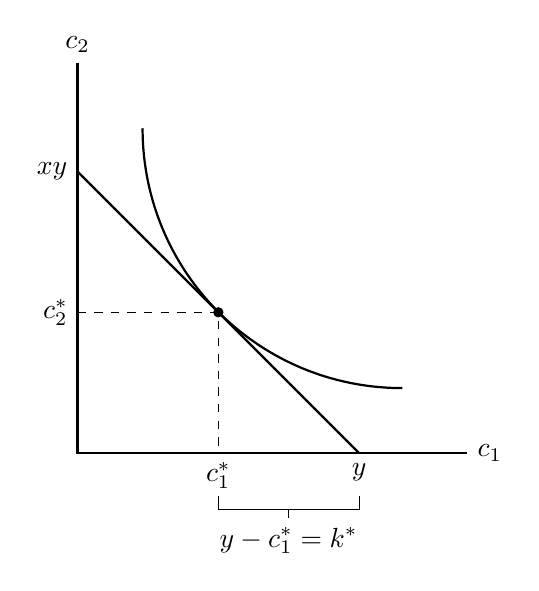
\begin{tikzpicture}[scale=0.55]
			\draw [thick] (0,6.5) node [left]{\( xy \)} to (6.5,0) node [below]{\( y \)};
			\draw [thick] (0,9) node[above]{\(c_2\)} -- (0,0) -- (9,0) node[right]{\(c_1\)};
			\draw [dashed] (0,3.25) node[left]{\(c_2^*\)} -- (3.25,3.25) -- (3.25,0) node[below]{\(c_1^*\)};
			\filldraw [black] (3.25,3.25) circle (3pt);
			\draw [thick] (1.5,7.5) to [out=-90,in=180] (7.5,1.5);
			\draw (3.25,-1) -- (3.25,-1.3) -- (6.5,-1.3) -- (6.5,-1);
			\draw (4.875,-1.3) -- (4.875,-1.5) node [below] {\( y-c_1^*=k^* \)};
		\end{tikzpicture}
	\end{figure}
	\begin{itemize}
		\item The individual chooses \( (c_1,c_2) \) such that the indifference curve is tangent to the budget constraint. The optimal choice of \( k^* \) is
		\[
			k^* = y - c_1^*
		\]
		\item This simple model assumes that the marginal product of capital is a constant \( x \). A more realistic assumption is that capital exhibits a ``diminishing marginal product''. Let \(f(k)\) denote a general production function. In general, \( f'(k)>0 \). A diminishing marginal product of capital means that
		\[
			f''(k) < 0
		\]
	\end{itemize}
	\begin{figure}[H]
		\centering
		\begin{tikzpicture}[scale=0.55]
			\draw [thick] (0,9) node[above]{\( f(k) \)} -- (0,0) -- (9,0) node [right]{\(k\)};
			\draw [thick] (1,1) .. controls (1.25,6) and (4,7.75) .. (8,8);
			\node at (8.5,8.5) {\( f(x) \)};
		\end{tikzpicture}
		\begin{tikzpicture}[scale=0.55]
			\draw [thick] (0,9) node[above]{\( f'(k) \)} -- (0,0) -- (9,0) node [right]{\(k\)};
			\draw [thick] (1,8) .. controls (1.25,3) and (2.5,1.25) .. (8,1);
			\node at (9,1) {\( f'(x) \)};
		\end{tikzpicture}
	\end{figure}
\subsection{A Model with Private Debt}
	\begin{itemize}
		\item Consider private debt as IOUs issued by individuals -- private loans. Let there be two types of individuals:
		\begin{itemize}
			\item borrowers: endowed with nothing when young and \(y\) units of goods when old;
			\item lenders: endowed with y units of goods when young and nothing when old.
		\end{itemize}
		\item In each generation, half of the people are borrowers and the rest half are lenders.
		\item To begin with, suppose that private debt is the only asset in the economy. \textbf{There is neither money nor capital.}
		\item For a lender,
		\begin{itemize}
			\item the first-period budget constraint is
			\[
				c_{1,L} + l \leq y,
			\]
			where \( l \) demontes the amount of loans;
			\item the second-period budget constraint Is
			\[
				c_{2,L} \leq rl,
			\]
			where \( r \) is the gross, real interest on loans;
			\item the lifetime budget constraint is
			\[
				c_{1,L} + \frac{c_2,L}{r} \leq y.
			\]
			by combining the two period budget constraints.
		\end{itemize}
		\item We can depict the lender's lifetime budget constraint.
	\end{itemize}
	\begin{figure}[H]
		\centering
		\begin{tikzpicture}[scale=0.45]
			\draw [thick] (0,5.1) node [left]{\( \substack{ry\\(r<1)} \)} -- (11,0) node [below] {\( y \)};
			\draw [thick] (0,7.9) node [left]{\( \substack{y\\(r=1)} \)} -- (11,0);
			\draw [thick] (0,10.3) node [left]{\( \substack{ry\\(r>1)} \)} -- (11,0);
			\draw [thick] (0,11) node[above]{\(c_{2,L}\)} -- (0,0) -- (14,0) node[right]{\(c_{1,L}\)};
			\draw [dashed] (4.7,-4.1) -- (4.7,5.9);
			\draw (4.7,-3.9) -- (4.7,-4.1) -- (11,-4.1) -- (11,-3.9);
			\draw (7.85,-4.1) -- (7.85,-4.3) node [below] {\( i^* (r>1) \)};
			\draw [dashed] (5.1,-2.7) -- (5.1,4.2);
			\draw (5.1,-2.5) -- (5.1,-2.7) -- (11,-2.7) -- (11,-2.5);
			\draw (8.05,-2.7) -- (8.05,-2.9) node [below] {\( i^* (r=1) \)};
			\draw [dashed] (6.3,0) node [below]{\( c_{1,L}^* \)} -- (6.3,2.3);
			\draw (6.3,-1.1) -- (6.3,-1.3) -- (11,-1.3) -- (11,-1.1);
			\draw (8.55,-1.3) -- (8.55,-1.5) node [below] {\( i^* (r<1) \)};
			\draw [thick] (11.5,1) to [out=-180,in=-90] (1,10);
			\draw [thick] (12.5,2) to [out=-180,in=-90] (2,10);
			\draw [thick] (13.5,3) to [out=-180,in=-90] (3,10);
		\end{tikzpicture}
	\end{figure}
	\begin{itemize}
		\item The lender chooses \((c_1, c_2)\) such that the indifference curve is tangent to the budget constraint.
		\item We assume that preferences are such that as \(r\) increases, \( c_{1,L} \) decreases so that \( l \) increases. Let \( L \) denote the aggregate supply of loans.
	\end{itemize}
	\begin{figure}[H]
		\centering
		\begin{tikzpicture}[scale=0.55]
			\draw [thick] (0,9) node[above]{\(r\)} -- (0,0) -- (9,0) node [right] {Goods};
			\draw [thick] (1,1) .. controls (4,2) and (7,4) .. (8,8);
			\node at (7.5,8.5) {Supply of loans};
		\end{tikzpicture}
	\end{figure}
	\begin{itemize}
		\item For a borrower,
		\begin{itemize}
			\item the first-period budget constraint is
			\[
				c_{1,B} \leq b,
			\]
			where \( b \) denotes the amount of debt (loans);
			\item the second-period budget constraint is
			\[
				c_{2,B} \leq y - rb
			\]
			\item the lifetime budget constraint is
			\[
				c_{1,B} + \frac{c_{2,B}}{r} \leq \frac{y}{r}.
			\]
			by combining the two period budget constraints.
		\end{itemize}
		\item We can depict the borrower's lifetime budget constraint.
	\end{itemize}
	\begin{figure}[H]
		\centering
		\begin{tikzpicture}[scale=0.45]
			\draw [thick] (0,10.3) node [left]{\( y \)} -- (11,0) node [below]{\( \substack{y/r\\(r<1)} \)};
			\draw [thick] (0,10.3) -- (7.9,0) node [below]{\( \substack{y\\(r=1)} \)};
			\draw [thick] (0,10.3) -- (4.9,0) node [below]{\( \substack{y/r\\(r>1)} \)};
			\draw [thick] (0,11) node[above]{\(c_{2,B}\)} -- (0,0) -- (14,0) node[right]{\(c_{1,B}\)};
			\draw [dashed] (1.8,0) node [below]{\( c_{1,B}^* = b^* \)} -- (1.8,6.3);
			\draw [dashed] (3.4,0) -- (3.4,5.8);
			\draw [dashed] (4.7,0) -- (4.7,5.9);
			\draw [->] (1.8,2) -- (3.4,2);
			\draw [->] (3.4,2) -- (4.7,2);
			\draw [thick] (11.5,1) to [out=-180,in=-90] (1,10);
			\draw [thick] (12.5,2) to [out=-180,in=-90] (2,10);
			\draw [thick] (13.5,3) to [out=-180,in=-90] (3,10);
		\end{tikzpicture}
	\end{figure}
	\begin{itemize}
		\item The borrower chooses \((c_1, c_2)\) such that the indifference curve is tangent to the budget constraint.
		\item We assume that preferences are such that as \(r\) increases, \(c_{1,B}\) decreases so that \(b\) decreases. Let \(B\) denote the aggregate demand for loans.
	\end{itemize}
	\begin{figure}[H]
		\centering
		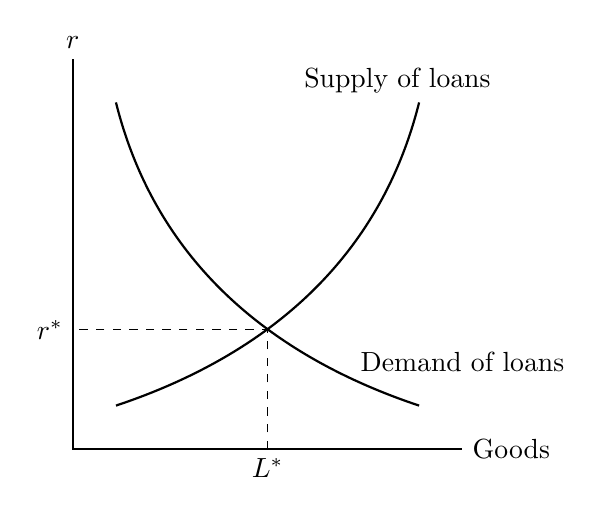
\begin{tikzpicture}[scale=0.55]
			\draw [thick] (0,9) node[above]{\(r\)} -- (0,0) -- (9,0) node [right] {Goods};
			\draw [thick] (1,1) .. controls (4,2) and (7,4) .. (8,8);
			\node at (7.5,8.5) {Supply of loans};
			\draw [thick] (1,8) .. controls (2,4) and (5,2) .. (8,1);
			\node at (9,2) {Demand of loans};
			\draw [dashed] (4.5,0) node [below]{\( L^* \)}-- (4.5,2.75) -- (0,2.75) node [left]{\( r^* \)};
		\end{tikzpicture}
	\end{figure}
\subsection{Rate of Return Equality}
	\begin{itemize}
		\item Suppose that we introduce capital to our model with private debt.
		\begin{itemize}
			\item The marginal product of capital is \( x \).
			\item The rate of return on loans is \( r^* \).
		\end{itemize}
		\item How should \textbf{lenders} choose between capital and private loans?
		\begin{itemize}
			\item What would happen if \( x > r^* \) ?
			\item What would happen if \( x < r^* \) ?
			\item What would happen if \( x = r^* \) ?
		\end{itemize}
		\item For people to be willing to hold both capital and loans as assets, we must have
		\[
			x = r
		\]
		or more generally
		\[
			f'(k) = r
		\]
		\item Suppose that there are many assets available to individuals. Without any uncertainty about returns and any government restrictions (\textbf{perfect substitutes}), the rate of return on these assets must be identical for people to hold all available assets simultaneously.
		\item We refer to this as the principle of ``\textbf{rate-of-return equality}''.
	\end{itemize}
\subsection{Coexistence of Money and Other Assets}
	\begin{itemize}
		\item If we introduce money into our model with capital and private debt, the rate-of-return equality requires that for all assets to be held by individuals,
		\[
			\frac{n}{z} = r = z
		\]
		Here \(n\) is the growth rate of population and \(z\) is the growth rate of money supply; so \(n/z\) is the rate of return on money.
		\item \textbf{If all assets are perfect substitutes}, then rate-of-return equality holds for all assets to coexist. In this case, how does money interact with other assets?
	\end{itemize}
\subsubsection{The Tobin Effect}
	\begin{itemize}
		\item Consider a standard OLG model with money and capital. Each young is endowed with \( y \) units of consumption goods when young and nothing when old.
		\item Suppose that capital displays a diminishing marginal product. That is, \( f''(k)<0 \).
		\item For both money and capital to be valued, we must have
		\[
			f'(k) = \frac{n}{z}
		\]
		For any given \( (n,z) \) we can find a desired level of capital stock.
		\item What if there is a permanent increase in \( z \)?
		\item Graphically, we show the determination of \( k \).
	\end{itemize}
	\begin{marginfigure}
		\centering
		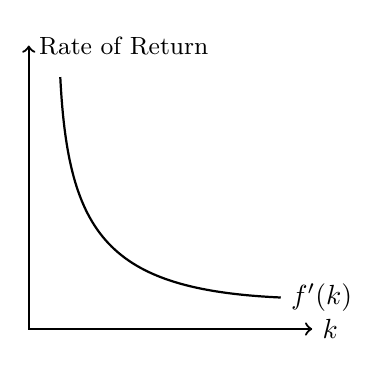
\begin{tikzpicture}[scale=0.4]
			\draw [thick, <->] (0,9) node[right]{\small{Rate of Return}} -- (0,0) -- (9,0) node [right]{\(k\)};
			\draw [thick] (1,8) .. controls (1.25,3) and (2.5,1.25) .. (8,1) node [right]{\( f'(k) \)};
		\end{tikzpicture}
		\caption{Tobin effect}
	\end{marginfigure}
	\begin{itemize}
		\item When \( z \) increases, \( n/z \) decreases and \( k^* \) increases.
		\item The substitution of capital for money in reaction to an increase in inflation, described by Tobin (1965), is called the ``\textbf{Tobin effect}''.
		\item Does the Tobin effect suggest that an increase in \( z \) could help to increase output? In our model, the output in period \( t \) is
		\[
			GDP_t = N_ty + N_{t-1}f(k_{t-1}).
		\]
		If we live in a world \textbf{where money and capital are perfect substitutes, an increase in} \(z\) \textbf{would raise }\(k\) \textbf{and hence output}. Should the policy maker use \(z\) as a tool to raise output?
		\begin{itemize}
			\item Output \( \neq \) Welfare.
			\item The Tobin effect is not large in the real world.
		\end{itemize}
	\end{itemize}
\subsection{The Golden Rule Capital Stock}
	\begin{itemize}
		\item Let the feasible set be
		\[
			N_t c_{1,t} + N_{t+1} c_{2,t} + N_t k_t \leq N_t y + N_{t-1} f(k_{t-1})
		\]
		Dividing by \( N_t \) to find the feasible set for per person. If we also restrict ourselves to stationary solutions, we can elimiate the time subscriptss. These simplifications results in
		\[
			c_1 + \frac{c_2}{n} + k \leq y + \left[ \frac{f(k)}{n} \right]
		\]
		or
		\[
			c_1 + \frac{c_2}{n} \leq y + \left[ \frac{f(k)}{n} - k \right]
		\]
	\end{itemize}
	\begin{figure}[H]
		\centering
		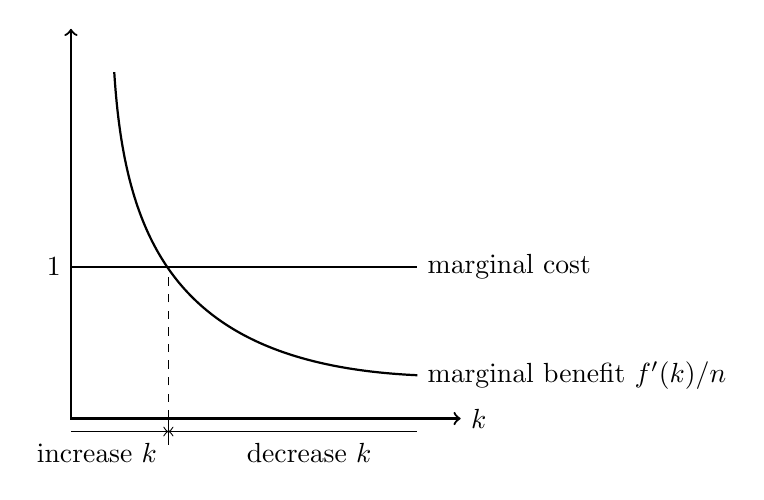
\begin{tikzpicture}[scale=0.55]
			\draw [thick, <->] (0,9) -- (0,0) -- (9,0) node [right]{\(k\)};
			\draw [thick] (0,3.5) node [left]{\( 1 \)} -- (8,3.5) node [right]{marginal cost};
			\draw [dashed] (2.25,0) -- (2.25,3.5);
			\draw [] (2.25,0) -- (2.25,-0.6);
			\node at (0.6,-0.8) {increase \( k \)};
			\draw [->] (0,-0.3) -- (2.25,-0.3);
			\node at (5.5,-0.8) {decrease \( k \)};
			\draw [<-] (2.25,-0.3) -- (8,-0.3);
			\draw [thick] (1,8) .. controls (1.25,4) and (2.5,1.25) .. (8,1) node [right]{ marginal benefit \( f'(k)/n \)};
		\end{tikzpicture}
	\end{figure}
\subsection{When Money and Other Assets are not Perfect Substitutes}
	\begin{itemize}
		\item In the real world, fiat money and other assets \textbf{are not perfect substitutes}. In particular, the rate of return on money is generally lower than the rate of return on other assets. What are the effects of anticipated inflation on interest rate, capital and output?
		\item This raises an obvious question: why would money still be valued? We postpone this question for later sections. For now, consider a simple argument: legal restriction. Each young is required by law to acquire money worth a fixed number of goods \( q^* \)
		\item Nominal interest rate and real interest rate.
		\begin{itemize}
			\item \textbf{Nominal} interest rates: the number of \textbf{dollars} paid in interest for each dollar lent.
			\item \textbf{Real} interest rates: the number of \textbf{goods} paid in interest for each good lent.
			\item Nominal interest rates are the ones cited by financial intermediaries and the press.
			\item In times of inflation, nominal intrest rates do not reflect the real rate of return.
			\item Let \( R_t \) and \( r_t \) denoate the nominal interest rate and the real interest rate. Let \( p_t \) denote the price of a good.
		\end{itemize}
		\item We can express the gross interest rate \( r_t \) as
		\begin{equation}
			r_t = \frac{R_tp_t}{p_{t+1}} = R_t\frac{p_t}{p_{t+1}} \label{E:5.1}
		\end{equation}
		If we arrange \cref{E:5.1}, we can obtain
		\[
			\underbrace{R_{t-1}}_{\substack{\text{net nominal}\\\text{interest rate}}} = \underbrace{(r_t - 1)}_{\substack{\text{net real}\\\text{interest rate}}} + \underbrace{\left(\frac{p_{t+1}}{p_t} - 1\right)}_{\text{net inflation rate}} + (r_t -1)\left(\frac{p_{t+1}}{p_t} - 1\right)
		\]
		\item For low values of the real interest rate and the inflation rate, we have approximately:
		\begin{center}
			net nominal interest rate = net real interest rate + net inflation rate.
		\end{center}
		\item \textbf{Anticipated inflation and the nominal interest rate:} the predicted full adjustment of the nominal interest rate to anticipated inflation is called the ``\textit{Fisher effect}'' - named after Irving Fisher
		\item Consider a model with moneym capital and private debt. Suppose that the marginal product of capital is \( x \). The rate-of-return equality implies that
		\[
			x = r_t = R_t\frac{p_t}{p_{t+1}}
		\]
		Note that here money is held by people \textbf{because of the legal restriction. The rate-of-return equality applies to capital and private debt}. As the rate of return on money is \( p_t/p_{t+1} = n/z \), we have
		\[
			x = R_t\frac{n}{z} \quad \text{or} \quad R_t=x\frac{z}{n}
		\]
		\item The real interest rate is a constant \( x \). The nominal interest rate rises with anticipated inflation to keep the real interest rate constant \( x \).
		\item There is a tendency for nominal interest rates and inflation rates to move together in accordance with the Fisher effect. However, the gap between the nominal interest rate and the inflation rate is not cosntant due to changes in the real interest rate.
		\item Will inflation affect the real interest rate?
		\begin{itemize}
			\item In our previous example,
			\[
				x = r_t = R_t \frac{n}{z}.
			\]
			The real interest rate is always a constant \( x \) by the rate-of-return equality. An increases in inflation will only affect the nominal interest ratem but not the real interest rate. The key assumption is a constant marginal product of capital.
			\item What if capital exhibits a diminishing marginal product?
		\end{itemize}
		\item \textbf{Anticipated inflation and the real interest rate:} an exception to the Fisher effect could occur \textbf{if money, private debt, and capital are subsitutes and capital has a diminshing marginal product.}
		In this case,
		\begin{itemize}
			\item an increase in the inflation rate leads to an increase in capital - the Tobin effect;
			\item an increase in capital lends to a decline in the real interest rate because of diminishing marginal product of capital;
			\item overall, an increase in inflation will still lead to a rise in the nominal interest rate, however, beacuse of the simultaneous decrease in the real interest rate, the nominal interest rate will not rise by the full amount of the rise in inflation.
		\end{itemize}
	\end{itemize}
\subsection{Risk}
	\begin{itemize}
		\item So far, we have assumed that all assets pay a rate of return that is known with complete certainty. What would happen to rate-of-return equality if instead one asset has a random rate of return?
		\begin{itemize}
			\item For example: there is some positive probability that a loan will not be repaid by the borrower. If the marginal product of capital is a constant \( x \), then capital and private debt are \textbf{not} perfect substitutes.
		\end{itemize}
		\item If people do not care about risk (are ``risk neutral''), then the rate-of-return equality still holds on average. Suppose that an asset pays return \( r_1,r_2,\dots, r_n \) with probabilities \( \pi_1,\pi_2,\dots,\pi_n, \)respectively. The expected rate of return on this asset can be calculated as
		\[
			E(r) = \pi_1r_1 + \pi_2r_2 + \cdots + \pi_nr_n
		\]
		The rate-of-return equality is modified to
		\[
			E(r) = x
		\]
		\item Are people risk neutral? Probability not.
		\item If people are risk averse, people may still accept a risky asset. However, the rate-of-return equality will not hold in this case. In fact, the expected rate of return on this risky asset must exceed that of the risk-free asset, compensating for the risk.
		\item The extra average rate of return that is necessary to entice people to hold a risky asset is called a risk premium,
		\[
			\text{risk premium} = E (r_\text{risky}) - r_\text{safe}
		\]
		The greater the potential loss and the greater the probability of the loss, the larger the risk premium must be.
		\item In many real economies, why do people choose to hold fiat money when many alternative assets appear to offer greater rates of return?
	\end{itemize}
\section{Liquidity and Financial Intermediation}
\subsection{Introduction}
	\begin{itemize}
		\item We have discussed why money is valued in many real economies in which other assets have a greater return than money:
		\begin{itemize}
			\item risk premium
		\end{itemize}
		\item In this section, we consider an additional explanation that money is valued despite its low return: liquidity.
		\begin{itemize}
			\item Money is a liquid asset.
			\item Illiquid assets offer a higher rate of return than liquid assets. 
			\item Financial intermediation could emerge by borrowing at a low rate of return while investing at a high rate of return.
		\end{itemize}
	\end{itemize}
\subsection{Money as a Liquid Asset}
	\begin{itemize}
		\item People might hold money and other assets for different motives.
		\begin{itemize}
			\item Why do people hold money?
			\item Why do people hold assets such as houses?
		\end{itemize}
		\item Compared with other assets, money
		\begin{itemize}
			\item change hands much more frequently;
			\item is held for shorter periods of time;
			\item is less costly to exchange.
		\end{itemize}
		\item We say that an asset is ``liquid'' if it is exchanged easily, quickly, and at little cost. Money is the most liquid asset.
	\end{itemize}
\subsection{A Model of Illiquidity}
	\begin{itemize}
	\item We develop a model based on Freeman (1985) to capture the essential distinctions between liquid and illiquid assets. The model is consistent with the following observations:
		\begin{enumerate}[label=\textbf{\arabic*.}]
			\item money and capital are both valued;
			\item the rate of return of capital exceeds that of money;
			\item money is exchanged more often than capital.
		\end{enumerate}
		\item Consider an economy of overlapping generations in which people live for three periods: young, middle age and old.
		\item People are endowed with \( y \) units of the consumption good when young and nothing in the other two periods of life. Preferences are such that people value consumption in all three periods.
		\item Let \( N_t \) represent the number of people in the generation born at time \( t \), with \( N_t = nN_{t-1} \).
		\item There is a constant supply of money \( M \) in the economy. Money is distributed equally among the initial middle-aged individuals.
		\item There is a single physical asset, capital.
		\begin{itemize}
			\item A unit of capital may be created from a unit of the consumption good in any period \( t \).
			\item Capital may be created in any amount.
			\item Two periods after capital is created, a unit of capital produces \( X \) units of the consumption goods and then fully depreciates. Let \( X > n^2 \)
			\item Each initial old begins with a stock of capital that produces \( Xk_0 \) goods in the first period.
		\end{itemize}
		\item Two assumptions about information: we assume that
		\begin{itemize}
			\item it is expensive/impossible to observe the capital created by others, which implies capital cannot be traded in the 2nd period of life for consumption -- capital is illiquid.
			\item it is impossible to enforce repayment of IOUs because people can costlessly hide from anyone looking for them and in this way avoid repaying their IOUs -- no private debt.
		\end{itemize}
		\item The second assumption ensures that private borrowing and lending is not feasible in this economy. We will relax this assumption later.
		\item Let \( c_{1,t},c_{2,t+1},c_{3,t+2} \) denote the consumption in the first, second and third periods of life for an individual born in period \( t \), respectively.
		\item Given the pattern of endowments, individuals need to find ways to provide consumption in the second and third periods of their lives. Individuals can choose between capital and money.
		\begin{itemize}
			\item Second period: can use only money.
			\item Third period: can use both money and capital. Should an individual use capital or money to finance the third-period consumption?
			\begin{itemize}
				\item If the individual holds money from the first period to the third period, the two-period rate of return of money is
				\[
					\frac{v_{t+2}}{v_t} = \frac{v_{t+2}}{v_{t+1}}\frac{v_{t+1}}{v_t} = n^2
				\]
				\item If the individual holds capital from the first period to the third period, the two-period rate of return of capital is \( X \).
				\item Which asset would the individual choose to hold to finance the third-period consumption?
			\end{itemize}
		\end{itemize}
		\item We can summarise the budget constraints faced by the individual as
		\begin{itemize}
			\item the first-period budget constraint
			\[
				c_{1,t} + v_tm_t + k_t \leq y,
			\]
			\item the second-period budget constraint
			\[
				c_{2,t+1} \leq v_{t+1}m_t
			\]
			\item the third-period budget constraint
			\[
				c_{3,t+2} \leq Xk_t
			\]
			\item Combining the three period budget constraints, we have
		\end{itemize}
		\begin{align*}
			c_{1,t} + \frac{v_t}{v_{t+1}}c_{2,t+1} + \frac{1}{X}c_{3,t+2} &\leq y,\\
			\text{or } c_{1,t} + \frac{1}{n}c_{2,t+1} + \frac{1}{X}c_{3,t+2} &\leq y
		\end{align*}
		\item The frontier of the budget set would be a plane in a three-dimensional space. The optimal \( c_{1,t}^*,c_{2,t+1}^*,c_{3,t+2}^* \) combination would be located where an indifference curve is tangent to this plane.
		\item Some observations from the model:
		\begin{enumerate}[label=\textbf{\arabic*.}]
			\item money and capital are both valued -- money is used to finance the second-period consumption while capital is used to finance the third-period consumption;
			\item the rate of return of capital exceeds that of money -- the rate of return on capital is \( X \), which is greater that the rate of return of money \( n^2 \);
			\begin{itemize}
				\item the rate of return of equality is violated: because money and capital are not perfect subsitutes;
				\item Money: liquid. Capital: illiquid
			\end{itemize}
			\item money is exchanged more often than capital -- how should we compare the trading frequency of these two assets?
		\end{enumerate}
		\item Define the velocity of an asset as the amount of the asset that is exchanged in a given period of time divided by the total stock of that asset.
		\begin{itemize}
			\item In any period \( t \), the total stock of money change hands. It implies that eh velocity of money is 1.
			\item If we view a young individual's creation of capital as an exchange, the amount of new capital created in period \( t \) is \( N_tK_t \). The total stock of capital in period \( t \) is \( N_tk_t + N_{t-1}k_{t-1} \). The velocity of capital is thus
			\[
				\frac{N_tk_t}{N_tk_t + N_{t-1}k_{t-1}} < 1
			\]
			In this simple case that the total capital stock does not change in size over time, the velocity of capital is 1/2.
			\item It verifies that the velocity of money is higher than the velocity of capital.
		\end{itemize}
	\end{itemize}
\subsection{The Business of Banking}
	\begin{itemize}
		\item Suppose that now at least some people cannot hide from their creditors so that enforcement of their IOUs is possible. \( \rightarrow \) This allows the emergence of banking and a new form of liquid asset -- private debt (IOUs).
		\item Suppose that you are the only one in the economy who can issue IOUs. How might you use your ability to make profits?
	\end{itemize}
\subsubsection{A Simple Arbitrage Plan}
	\begin{itemize}
		\item Here is a plan:
		\begin{itemize}
			\item In period \( t \), borrow one good from the young in period \( t \) (and issue a one-period IOU) and invest the good in the creation of capital. To induce the young to lend, you need to promise to pay the rate of return at least \( n \) (rate of return on money)
			\item In period \( t+1 \), repay \( n \) to your lender (and take back the one-period IOU issued at period \( t \)) by borrowing \( n \) from the young born in period \( t+1 \) ( and issuing another one period IOU). To induce the young to lendm you need to promise to pay thre rate of return at least \( n \).
			\item In period \( t+2 \), repay \( n \times n = n^2 \) to your lender (and take back the one-period IOU issued at period \( t+1 \)) from production using capital. total output produced is \( X \). Net profit is \( X-n^2 > 0 \)
		\end{itemize}
		\item In this case, you are essentially a third party that channels economy's saving to assets with the highest rate of return
	\end{itemize}
\subsubsection{The Effect of Arbitrage on Equilibrium}
	\begin{itemize}
		\item Suppose that you are not the only one that is able to ussye IOUs. A large number of competitive people (labelled as banks or intermediaries) can borrow goods from the younf (by costlessly issuing IOUs) and invest the goods in capital creation. How does this affect our equilibrium outcome> In particular, what will the one-period rate of return (call it \( r \)) paid on these IOUs in a competitive equilibrium be?
		\begin{itemize}
			\item If you are the only one that issues IOUs, the one-period interest rate on IOUs is \( r = n \). (The minimum rate to entice lenders to lend.)
			\item With a large number of people issuing IOUs, they compete for lenders till \( r=X^{1/2} \). Then there eill be no incentive for intermediaries to offer higher interest rates on IOUs. Perfectly competitive intermediaries drive their profits to 0. 
		\end{itemize}
		\item In the absence of financial intermediation, capital was held only to acquire consumption in the third period of life; money was held to acquire consumption in the second period of life.
		\item With financial intermediation, IOUs (inside money) replaces money (outside money) in the acquisition of consumption in the second period of life. Inside money: ``money'' issued by private financial intermediaries. Outside money: fiat money issued by central bank.
		\begin{itemize}
			\item People invest in capital directly to acquire consumption in the third period of life.
			\item People invest in capital indirectly through intermediaries to acquire consumption in the second period of life.
		\end{itemize}
		\item Financial intermediation serves to mobilize all the savings of the economy for investment in the asset that generates a greater rate of return. It implies that output will be higher in an economy with financial intermediation.
		\item In terms of welfare, all future generations benefit. Only the initial middle-aged are worse off (money loses value as people abandon it).
	\end{itemize}
\subsection{Summary}
	This section focuses on models where money and other assets are \textbf{not} perfect substitutes.
	\begin{itemize}
		\item In the model of illiquidity, money serves as the liquid asset and capital serves as the illiquid asset. Money earns a lower rate of return, but is exchanged more frequently.
		\item If some people can issue private IOUs, financial intermediaries naturally emerge to take advantage of the rate-of-return differences in money and capital. These intermediaries provide a service by correcting the mismatch of maturities between liquid money and illiquid capital.
		\item There are other roles for banks or financial intermediaries
		\begin{itemize}
			\item Banks serve as monitors of risky investment: diversification and lower monitoring cost.
			\item Banks allow people to insure each other.
			\item Banks can help reduce the cost of evaluating loans.
			\item Banks can enjoy other economies of scale.
		\end{itemize}
	\end{itemize}
\section{Bank Risk}
\subsection{Introduction}
	\begin{itemize}
		\item In our model of banks, banks take deposits and invest in interest-bearing assets. Are there any risk that banks face?
		\item In the real world, there are many instances of bank failures.
		\item In this chapter, we focus on two possible reasons for bank failures:
		\begin{itemize}
			\item a sudden rush of withdrawals;
			\item unexpectedly low return on interest bearing assets.
		\end{itemize}
	\end{itemize}
\subsection{A Model of Demand Deposit Banking}
	\begin{itemize}
		\item Banks have liabilities that are payable on demand but assets that are not. This mismatch of bank assets and liabilities raises the possibility of a ``bank panic'' or ``bank run''.
		\begin{itemize}
			\item If depositors all withdraw at once, a bank must borrow or sell its assets to pay them off.
			\item If all depositors fear that the rush of others to withdraw will leave them with nothing, they will rationally join the rush. This is called a ``bank run''.
		\end{itemize}
		\item Assume that \( N \) three-period-lived individuals are born each period (in overlapping generations).
		\item Each individual is endowed with \( y \) units of consumption goods only when young.
		\item No one consumes when young. Everyone wants to consume in one of the next two periods of life, depending on their type.
		\begin{itemize}
			\item Early consumer: with 0.5 probability, the young becomes a type 1, who consumes in the second period of life.
			\item Late consumer: with 0.5 probability, the young becomes a type 2, who consumes in the third period of life.
		\end{itemize}
		\item No one knows his type when young. Everyone learns his type in the second period of life. \textbf{An individual's type is not observed by anyone else, including banks.}
		\item Individuals have access to two assets: storage and capital
		\begin{itemize}
			\item Storage: the gross rate of return is 1 over one period.
			\item Capital: produces \( X \) goods for each good invested two periods after its creation, where \( X>1 \).
		\end{itemize}
		\item Early liquidation of capital: capital can be sold one period after its creation.
		\begin{itemize}
			\item The price is \( v^k \), where \( v^k\leq X \). (why this must be true?)
			\item There is a verification cost \( \theta \) per unit of capital. We assume \( 1+\theta > X \)
		\end{itemize}
		\item Assume that private IOUs are possible among members of the same generation, but not between generations.
		\item Effective rates of return on storage and capital:
		\begin{table}[H] \centering
			\begin{tabular}{|l|l|l|}
			\hline
			Effective rates of return on: & One Period 							  & Two Periods      \\ \hline
			Storage                       & \textbf{1} 							  & 1                \\ \hline
			Capital                       &  \( v^k-\theta \) (early liquidation) & \textbf{\( X \)} \\ \hline
			\end{tabular}
		\end{table}
		\item This structure of returns ensures that \( v^k-\theta <1 \)
		\item \textbf{Individuals do not know their type at the time he chooses his asset.} How should individuals select assets to save for future consumption?
		\begin{itemize}
			\item Storage: offers a \textbf{better} one-period return, but \textbf{worse} two-periods return.
			\item Capital: offers a \textbf{worse} one-period return, but \textbf{better} two-periods return.
		\end{itemize}
		\item Suppose that there exist banks. Banks know that in each generation, half of its people will be of each type. If all individuals deposit their endowments at the bank, the bank can invest half of its deposits \( Ny/2 \) in storage and half in capital. A bank can offer the rate of return on deposits
		\begin{itemize}
			\item 1 after one period;
			\item X after two periods.
		\end{itemize}
		\item Individuals enjoy the higher rate of return in both periods.
		\item Banks provide liquidity by taking advantage of the fact that there is more randomness for an individual than for the aggregate economy.
		\item In our model, the bank provides demand deposits: the bank relies on the word of the depositor and make returns available to any depositor who asks for them. Would all depositors tell the truth?
		\begin{itemize}
			\item Type 1 people will not pretend to be type 2.
			\item Type 2 people do not want to claim to be type 1: if they do so, they will withdraw their deposits earlier and store the goods by themselves. Overall, the rate of return is 1, which is less than \( X \).
		\end{itemize}
	\end{itemize}
\subsection{Bank Runs}
	\begin{itemize}
		\item Suppose you are a type-2 consumer and now you hear a \textbf{rumor} that every other type 2 is going to pretend to be type 1 in order to withdraw his deposits from the bank. Would you rush to the bank and try to withdraw early?
		\begin{itemize}
			\item The bank has \( Ny/2 \) in storage which allows the bank to payoff \( N/2 \) people. Each withdraws \( y \) units of goods.
			\item If you do not withdraw and a large number of type 2 withdraw early, the bank has to sell some of its capital to meet the demand. For every 1 unit of capital sold, the bank receives \( v^k-\theta \) goods. Therefore, the total capital stock \( Nt/2 \) can be sold to pay off \( Ny \left( v^k-\theta \right)/2 \). Given that \( v^k-\theta<1 \), \textbf{the bank cannot pay off all type 2 people.} An honest type 2 may get nothing if everyone else withdraws early and he does not!
			\item If every type 2 believes that all others will rush to the bank to withdraw early, he will also rush to the bank to withdraw early.
			\item In this way, the bank would not be able to meet all its obligations and a bank run occurs.
		\end{itemize}
	\end{itemize}
\subsection{Preventing Panics}
	\begin{itemize}
		\item How can the bank in our model avoid the bank run? There are several ways that economists have identified.
		\item Interbank lending: if a bank faces a run can borrow enough to meet all withdrawals, it can avoid the losses from the sale of its capital.
		\begin{itemize}
			\item If a bank is threatened by a run, it could borrow from other banks or people who are not experiencing runs.
		\end{itemize}
		\item Identifying unnecessary withdrawals: if the bank can identify an individual's type, the bank can stop the bank run by refusing to allow type 2 people to withdraw early.
		\item Suspension of withdrawals: the bank can temporarily close its doors when its reserves of the liquid short-term asset (storage) have been used up, and then reopen in the next period when its long-term capital pays its return.
		\begin{itemize}
			\item If the bank follows such a policy, it will never be required to sell its capital at a loss.
			\item It follows that if a bank has the right to suspend withdrawals, it may never actually need to do so because depositors will no longer panic.
			\item An example: during the bank panics of 1893 and 1907, banks in the U.S. restricted convertibility of deposits into currency.
			\item This policy may not work well if the number of type 1 people is \textbf{random}.
		\end{itemize}
	\end{itemize}
\subsubsection{Government Deposit Insurance}
	\begin{itemize}
		\item Why should the government care more about bank failures?
		\item Government deposit insurance: the government can help prevent bank runs by guaranteeing type 2 people that they will receive their promised return even if the bank becomes insolvent.
		\begin{itemize}
			\item How can the government back up its guarantee? By taxing the endowment of the currently young generation.
			\item \textbf{If the government guarantee is believed by all people}, no type 2 would want to withdraw early. There will be no bank runs. In this case, the government will never have to use its power of taxation.
			\item The government guarantee prevents bank runs costlessly.
			\item The government may need to tax people to provide deposit insurance if
			\begin{itemize}
				\item the number of type 1 people is random and is unusually large;
				\item or if bank assets are risky.
			\end{itemize}
			\item In the U.S., the Federal Deposit Insurance Corporation (FDIC) gives the resolution costs of \$197.68 billion from 1980 to 1994.
		\end{itemize}
	\end{itemize}
\subsection{Bank Failures}
	\begin{itemize}
		\item The U.S. history of bank failures.
		\begin{itemize}
			\item From 1930 to 1933, bank failures averaged more than 2000 per year.
			\item From 1941 to 1981, bank failures averaged five per year.
			\item From 1982, bank failures rose and peaked at more than 200 failures in 1988
			\item From 2007, bank failures rose again.
		\end{itemize}
	\end{itemize}
	\begin{figure}[H]\centering
		\begin{tikzpicture}
			\begin{axis}[
				title = {Number of FDIC-insured commercial banks and trust},
				no markers,
				height = \axisdefaultheight,
				width = \textwidth,
				date coordinates in = x,
				date ZERO = {1960-01-01},
				xticklabel = {\year},
				xtick = {
					1940-01-01,	
					1950-01-01,
					1960-01-01,
					1970-01-01,
					1980-01-01,
					1990-01-01,
					2000-01-01,
					2010-01-01,
					2020-01-01
				},
				xmin = 1934-01-01,
				xmax = 2020-01-01,
				xtick pos = left,
				xtick align = outside,
				ytick = {0,50,100,150,200,250,300,350,400,450,500,550},
				ytick pos = bottom,
				ytick align = outside,
				ymin = 0,
				ymax = 550,
				legend pos = north east,
				legend cell align = left,
				]
				\addplot [color=myblue,thick,smooth] table [x=Date,y=Data,col sep=comma] {Bank Failures.csv};
			\end{axis}
		\end{tikzpicture}
	\end{figure}
	\begin{itemize}
		\item Government deposit insurance may actually induce banks to take greater risks than they would if they are not insured by the government -- Moral hazard of deposit insurance!
		\begin{table}[H]\centering
			\begin{tabular}{lrlr}
			\multicolumn{4}{c}{A Bank's  Balance Sheet} \\ 
			\multicolumn{2}{c|}{Assets}    & \multicolumn{2}{c}{Liabilities} \\ \hline
				Reserves & \multicolumn{1}{r|}{\( \gamma H \)}    				   & Deposits          & \( H \) \\
				Interest-bearing assets & \multicolumn{1}{r|}{\( (1-\gamma)H+W \)} & Net worth         & \( W \) \\ \hline
				Total assets & \multicolumn{1}{r|}{\( H+W \)}    				   & Total liabilities & \( H+W \)
			\end{tabular}
		\end{table}
		\item Deposits are protected from changes in the value of bank assets by the positive net worth of a bank. We use an example for an illustration.
		\item An example:
		\begin{table}[H]\centering
			\begin{tabular}{lrlr}
			\multicolumn{2}{c|}{Assets}    & \multicolumn{2}{c}{Liabilities} \\ \hline
				Reserves & \multicolumn{1}{r|}{\$2M}    			 & Deposits          & \$20M \\
				Interest-bearing assets & \multicolumn{1}{r|}{\$22M} & Net worth         & \$4M  \\ \hline
				Total assets & \multicolumn{1}{r|}{\$24M}    		 & Total liabilities & \$24M
			\end{tabular}
		\end{table}
		\item Suppose that the bank loses 5 percent of its interest-bearing assets because of an unexpected surge in loan defaults.
		\begin{table}[H]\centering
			\begin{tabular}{lrlr}
			\multicolumn{2}{c|}{Assets}    & \multicolumn{2}{c}{Liabilities} \\ \hline
				Reserves & \multicolumn{1}{r|}{\$2M}    			   & Deposits          & \$20M \\
				Interest-bearing assets & \multicolumn{1}{r|}{\$20.9M} & Net worth       & \$2.9M \\ \hline
				Total assets & \multicolumn{1}{r|}{\$22.9M}    		   & Total liabilities & \$22.9M
			\end{tabular}
		\end{table}
		\item Although the bank lost only 5\% of its interest-bearing assets, the shareholders lost 27.5\% (2.9/4=0.725) of their investment in the bank because the entire loss is subtracted from net worth.
		\item What if the bank loses 20 percent of its interest-bearing assets?
		\begin{table}[H]\centering
			\begin{tabular}{lrlr}
			\multicolumn{2}{c|}{Assets}    & \multicolumn{2}{c}{Liabilities} \\ \hline
				Reserves & \multicolumn{1}{r|}{\$2M}    			   & Deposits          & \$20M \\
				Interest-bearing assets & \multicolumn{1}{r|}{\$17.6M} & Net worth       & \$0 \\ \hline
				Total assets & \multicolumn{1}{r|}{\$19.6M}    		   & Total liabilities & \$20M
			\end{tabular}
		\end{table}
		\item Insolveny occurs since there are not enough assets to pay off the liabilities.
	\end{itemize}
\subsection{Moral Hazard of Deposit Insurance}
	\begin{itemize}
		\item A bank that takes on too much risk will be unable to attract shareholders or depositors.
		\item How will a bank attract depositors if there is government depositor insurance?
		\begin{itemize}
			\item If the government insures depositors against all losses, depositors will no longer be exposed to risk.
			\item Depositors will care about only return.
			\item Therefore, banks have an incentive to offer high return to attract depositors.
			\item High return is generally associated with high risk.
			\item A \textbf{moral hazard} problem of insurance.
		\end{itemize}
	\end{itemize}
\subsection{Importance of Capital Requirement}
	\begin{itemize}
		\item What can the government do to limit the risk taking that deposit insurance encourages?
		\item A ``capital requirement'' forces banks to maintain a net worth no less than some fraction of their assets.
		\begin{itemize}
			\item Capital requirement provides a cushion to absorb asset losses before depositors or the insurer of the deposits suffers any losses.
		\end{itemize}
		\item For example, the US government increased the core capital requirements from 3 percent of total assets to \textbf{8} percent in 1989;
	\end{itemize}
\subsection{Summary}
	In this section, we
	\begin{itemize}
		\item examined two sources of bank failures: runs on banks and bank holding risky assets;
		\item analyzed four ways that banks or the government can prevent bank runs;
		\item identified the moral hazard problem associated with government deposit insurance;
		\item Notice that so far our model of banks does not have money. The available assets are storage and capital. We proceed to the next section to include money and discuss the bank risk in a banking model with money.
	\end{itemize}
\section{Liquidity Risk and Bank Panics}
\subsection{Introduction}
	\begin{itemize}
		\item Our previous model of bank run: there is no money in the model economies -- the model economy focused on real factors.
		\item In the real economy: liquidity shortages, in the form of too little money (cash), are frequently associated with widespread bank failures, which can turn into bank panics.
		\item In this section, we develop a model where money and bank panics are clearly linked. We will use the model to examine
		\begin{itemize}
			\item how money withdrawals are associated with bank panics;
			\item the optimal monetary policy.
		\end{itemize}
	\end{itemize}
\subsection{A Model of Random Relocation}
	\begin{itemize}
		\item There are two islands: island 1 and island 2.
		\item On each island, \( N \) (a large number) of two-period lived individuals are born in each period. In the first period, each island has \( N \) initial old who live only in the first period.
		\item Each individual is endowed with \( y \) units of a perishable consumption good when young and nothing when old.
		\item Each individual wants to consume \textbf{only when old}.
		\item When born, each individual faces a risk that he will spend the second period of life on the other island. Each young is notified whether he will be relocated or not at the beginning the second period of life. For a young individual,
		\begin{itemize}
			\item With probability \( \pi \), he will be relocated to the foreign island.
			\item With probability \( 1 - \pi \), he will stay on the home island.
		\end{itemize}
		\item We assume that the relocation probability is the same on both islands. In aggregate, \( \pi N \) individuals will move from island 1 to island 2 and vice versa.
		\item Money: there is a central monetary authority that controls the money supply.
		\begin{itemize}
			\item In period \( t \), let \( M_t \) denote the aggregate supply of money.
			\item Money supply grows at a constant rate, \( M_t = zM_{t-1} \). Newly created money is used to finance a lump-sum transfer to young individuals.
		\end{itemize}
		\item Capital: capital matures in one period with the marginal product \( x \). We assume that \( x > \frac{v_{t+1}}{v_t} \), but
		\begin{itemize}
			\item it cannot move across locations;
			\item there is limited communication across islands, which renders claims against capital worthless.
		\end{itemize}
	\end{itemize}
\subsubsection{Without Banks}
	\begin{itemize}
		\item Decisions of an individual who is born in period \( t \):
		\begin{itemize}
			\item when young, the individual has y units of good that will be divided between money and capital,
			\[
				c_tm_t + k_t \leq y + \tau,
			\]
			where \( v_t \) denotes the value of money in period \( t \) and \( \tau \) denotes the lump-sum transfer from the government;
			\item when old, the individual's consumption depends on his relocation status:
			\begin{itemize}
				\item with probability \( \pi \), the individual is relocated and his second-period budget constraint is
				\[
					c^m \leq v_{t+1}m_t;
				\]
				\item with probability \( 1 - \pi \), the individual stays on the same island and his second period budget constraint is
				\[
					c^n \leq v_{t+1}m_t;
				\]
			\end{itemize}
		\end{itemize}
		\item Money market clearing condition
		\[
			v_tM_t = 2N(y+\tau-k_t);
		\]
		\item We focus on stationary allocations
		\[
			\frac{v_{t+1}}{v_t} = \frac{\frac{2N(y+\tau-k)}{M_{t+1}}}{\frac{2N(y+\tau-k)}{M_t}} = \frac{M_t}{M_{t+1}} = \frac{1}{z}
		\]
		\item Since we assume that individuals consume only when old, the young save everything to finance the second-period consumption. The young need to decide how to divide his saving between money and capital.
		\begin{itemize}
			\item If a young individual chooses to hold only money to finance his second-period consumption, we have
			\[
				c^m = c^n = v_{t+1}m_t = \frac{v_{t+1}}{v_t}(y+\tau) = \frac{y+\tau}{z}.
			\]
			\item If a young individual chooses to hold only capital to finance his second-period consumption, we have
			\[
				c^m = 0 \quad\text{and}\quad c^n = xk_t = x(y+\tau).
			\]
			\item Generally, a risk-averse young individual balances the risk against the return of each asset and acquires a combination of money and capital.
		\end{itemize}
		\item An individual's problem is
		\begin{alignat*}{2}
			\max_{m_t,k_t}\quad &&\pi u (c^m)&+(1-\pi) u (c^n)\\
			\text{s.t}\quad &&v_tm_t + k_t &\leq y + \tau\\
			&&c^m &\leq v_{t+1}m_t\\
			&&c^n &\leq v_{t+1}m_t + xk_t
		\end{alignat*}
		\item What is the individual's expected utility?
		\[
			\pi u (v_{t+1}m_t) + (1-\tau)u(v_{t+1}m_t+xk_t)
		\]
	\end{itemize}
\subsubsection{With Banks}
	\begin{itemize}
		\item Suppose that banks exist on each island. They can accept deposits and use the deposits to acquire assets.
		\item We assume that banks can identify who is a mover and who is a non-mover.
		\item How can banks help individuals achieve a better allocation?
		\begin{itemize}
			\item Imagine that young individuals deposit their endowments at the banks.
			\item On each island, the bank knows that a fraction of \( \pi \) people are movers and a fraction of \( 1 - \pi \) people are non-movers.
			\item After knowing whether to move, movers can go to the banks and withdraw their deposits under the rules established between the bank and the depositor.
			\item When old, movers finance their second-period consumption with money and non-movers finance their second-period consumption with capital.
		\end{itemize}
		\item After accepting the deposits, the bank's problem is to choose the combination of money and capital such that
		\begin{itemize}
			\item the asset allocation maximizes the expected utility of the individuals;
			\item there is enough money to meet the liquidity needs of the movers.
		\end{itemize}
		\item Formally, we consider the bank's decisions.
		\begin{itemize}
			\item On each island, the bank needs to decide how to allocate deposits between money and capital. The bank's balance-sheet constraint in period \( t \) is
			\[
				v_tm_t + k_t \leq y + \tau = d_t
			\]
			where \( d_t \) stands for the quantity of goods deposited by each individual.
		\end{itemize}
		\item Note that \( d_t,m_t,k_t \) in this balance-sheet constraint are expressed as per capita variables. We can define the reserve-to-deposit ratio \( \gamma = \frac{v_tm_t}{d_t} \)
		\item The bank's decisions
		\begin{itemize}
			\item The bank can pay movers up to the amount of real money balances that the bank possesses. Let \( r^m \) be the rate of return on deposits for movers. The deposit contract for movers is
			\[
				r^md_t = v_{t+1}\frac{m_t}{\pi} \quad\text{or}\quad r^m\pi d_t = v_{t+1}m_t.
			\]
			\item Let \( r^n \) be the rate of return on deposits for non-movers. The deposit contract for non-movers is
			\[
				r^nd_t = x\frac{k_t}{1-\pi} \quad\text{or}\quad r^n(1-\pi)d_t = xk_t.
			\]
			\item The bank chooses \( (m_t,k_t) \) and \( (r^m,r^n) \) to maximize the expected utility of an individual.
		\end{itemize}
		\item We rewrite an individual's budget constraints when there exist banks:
		\begin{itemize}
			\item when young, each individual deposits his endowment at the bank
			\[
				d_t \leq y + \tau,
			\]
			when old, a mover's budget constraint is
			\[
				c^m \leq r^m d_t,
			\]
			and a non-mover's budget constraint is
			\[
				c^n \leq r^n d_t.
			\]
		\end{itemize}
		\item The money market clearing conditions is unchanged.
		\item A bank's problem is
		\begin{equation*}
			\max_{m_t,k_t,r^m,r^n}\quad \pi u (c^m)+(1-\pi) u (c^n)
		\end{equation*}
		\begin{alignat*}{2}
			\text{s.t}\quad &&c^m &\leq v_{t+1}m_t\\
			&&c^n &\leq v_{t+1}m_t + xk_t\\
			&&v_tm_t + k_t &\leq y + \tau\\
			&&r^m\pi(y+\tau) &\leq v_{t+1}m_t\\
			&&r^n(1-\pi)(y+\tau) &\leq xk_t.
		\end{alignat*}
		\item Key features of the model with banks:
		\begin{itemize}
			\item important assumption -- banks \textbf{can costlessly} distinguish a mover from a non-mover;
			\item bank contract -- deposit contract distinguish between movers and non-movers;
			\item role of banks -- banks provide liquidity insurance for depositors.
		\end{itemize}
	\end{itemize}
\subsubsection{Comparison of the cases with and without Banks}
	\begin{itemize}
		\item Expected utility in the case with banks
		\[
			\pi u(r^md_t) + (1-\pi) u(r^nd_t)
		\]
		\item Expected utility in the case without banks
		\[
			\pi u(v_{t+1}m_t) + (1-\pi) u(v_{t+1}m_t+xk_t)
		\]
		\item Which one dominates?
		\begin{itemize}
			\item For non-movers
			\[
				\frac{v_{t+1}}{v_t}v_tm_t \leq \frac{v_{t+1}}{v_t} (y+\tau)
			\]
			\item For movers
			\[
				\frac{v_{t+1}}{v_t}v_tm_t + xk_t \leq x(y+\tau) 
			\]
			Hence expected utility of banks dominates for both non-movers and movers.
		\end{itemize}
	\end{itemize}
\subsection{Optimal Allocation}
	\begin{itemize}
		\item What is the optimal allocation in this economy? The planner maximizes aggregate welfare
		\[
			\pi u (c^m)+(1-\pi) u (c^n)
		\]
		subject to the resource constraint
		\[
			\pi c^m + (1-\pi)c^n + s = y+xs.
		\]
		\item Two observations: the planner
		\begin{itemize}
			\item should invest all endowment in capital;
			\item should not have a preference of one type over the other: perfect risk-sharing;
		\end{itemize}
		It follows that
		\[
			s = y \quad\text{and}\quad c^m=c^n=c^*= xy.
		\]
	\end{itemize}
\subsection{Optimal Allocation and Optimal Monetary Policy}
	\begin{itemize}
		\item What would monetary policy have to be to achieve perfect risk sharing?
		\begin{itemize}
			\item Recall that the deposit contract implies that
			\[
				c^m = r^md_t \quad\text{and}\quad c^n = r^nd_t.
			\]
			To achieve perfect risk sharing, we need to have
			\[
				r^m = r^n.
			\]
			One way to achieve this is to set the rate of return on money equal to the rate of return on capital
			\[
				\frac{1}{z} = x
			\]
			which is also labelled as the \textbf{Friedman rule}.
		\end{itemize}
		\item In general, the choice of the monetary policy that achieves full risk sharing \textbf{is not} the policy that achieves the most effcient allocation: it benefits the initial old.
		\item The monetary policy that maximizes welfare for all future generations is the one that keeps the money supply constant. The intuition follows from the OLG model of money.
		\begin{itemize}
			\item But the allocation associated with constant money supply may not achieve full risk sharing.
		\end{itemize}
		\item To summarize, to achieve full risk sharing, the optimal monetary policy is to set \( z = \frac{1}{x} \); to achieve the highest expected utility of all future generations, the optimal monetary policy is to set \( z=1 \).
	\end{itemize}
\subsection{Bank Risk}
	\begin{itemize}
		\item So far, there is no aggregate uncertainty. Banks do not have any risk. To consider bank risk, we modify our model and assume that \( \pi \) is a random variable.
		\begin{itemize}
			\item The fraction of people who move is drawn from a distribution of possible outcomes.
		\end{itemize}
		\item Suppose that the realisation of \( \pi \) could be
		\begin{itemize}
			\item with probability \( \epsilon \), a high fraction \( (\pi^H) \) of people are going to become movers;
			\item with probability \( 1 - \epsilon \), a low fraction \( (\pi^L) \) of people are going to become movers;
		\end{itemize}
		\item Let
		\[
			E(\pi) = \epsilon\pi^H + (1-\epsilon)\pi^L.
		\]
		\item How should a bank choose its portfolio then? The bank chooses the amount of money (cash reserve) in the presence of uncertain demand.
		\item Comparing an economy with a certain \( \pi \) and an economy with a random \( \pi \), we know that
		\begin{itemize}
			\item The bank will hold a larger amount of money in the uncertain environment. The reserve-to-deposit ratio is higher when \( \pi \) is random.
			\item Since capital offers a higher rate of return, the bank \textbf{will not choose} the amount of money to insure against the worst possible shock.
			\item The marginal condition balances the value of the insurance against uncertain demand with the opportunity cost of holding low-return money instead of high-return capital.
			\item With some probability, the bank's money holding could be too small to meet the realized liquidity demand. In case that the worst possible shock (highest demand for liquidity) is realised, the bank may not have enough cash reserve to meet the demand.
		\end{itemize}
	\end{itemize}
\end{document}